\chapter{ゲージ不変性とベクトルポテンシャルの必要性}

物理学を始める前に、実務的な事項が二つある。次回の講義は講師がベルギーに滞在するため休講となるが、講義は全十回が終わるまで続けられる。今夜の手書きノートも急遽用意された。これをクラス用ウェブサイトのためにスキャンしてくれる人がいれば、驚くほど遅いスキャナーからそのノートを救い出すことになる。

前回の講義は数学的に濃密であった。そうでないふりをするよりも、その中心的な計算をもう一度たどることにしよう。この講義の目的は、真の意味での理論的最小限、すなわち次の段階へ進むのに十分な構造を与えることである。物理学を失わずに数学を取り除くことができたなら、取り除くべき理由はいくらでもある。しかし厳密な法則は定量的な記述を要求し、定量的な記述は数学を要求する。記法は難解になるかもしれないが、それは物理学者が司祭的な言葉で主題を隠そうとしている証拠ではない。

おそらく、自然のより単純な定式化はまだ見つかっていないのであろう。ファインマンが冗談めかして言ったように、物理学のあらゆる方程式を二乗し、その二乗を足し合わせ、その和をゼロに等しいと置くことができる。そうすれば一つの方程式が得られる。なぜなら、そのときすべての二乗が消えなければならないからである。しかし、そこから新しい理解は生まれない。単純さとは、単に活字を圧縮することではなく、組織化する考え方を見出すことである。そのような考え方は若い誰かから来なければならないという示唆に聴衆の一人が異議を唱えたとき、その点はすぐに認められる。年齢は洞察とは無関係である。

\lectureoverview{まず、ローレンツスカラーを認識するために必要な添字記法を復習する。次に、相対論的理論のための四つの原理を定式化し、荷電粒子の導出を完全に繰り返し、最後にゲージ不変性を二度発見する。すなわち、作用における端点項として、そして電磁場テンソルの不変性としてである。}

\section{添字の言語再訪}

\subsection{なぜ一部の添字は上付きなのか}

\begin{equation}
x^\mu=(t,x,y,z),
\qquad
\mu=0,1,2,3,
\end{equation}
計量を
\begin{equation}
\eta_{\mu\nu}
=
\operatorname{diag}(-1,1,1,1).
\label{eq:sr7-metric}
\end{equation}
とする。座標と座標変位には上付き添字が割り当てられる：
\begin{equation}
dx^\mu=(dt,dx,dy,dz).
\end{equation}
それらの座標に関する微分には下付き添字が付く：
\begin{equation}
\partial_\mu
\equiv
\frac{\partial}{\partial x^\mu}.
\label{eq:sr7-gradient}
\end{equation}
どちらの族を上付きと呼び、どちらを下付きと呼ぶかは約束事であり、左と右という名が約束事であるのとよく似ている。しかし、いったん選んだならば、その約束事は一貫して従わなければならない。なぜなら、二つの族は異なる変換をするからである。

\begin{classroomqa}
\audiencequestion{添字はいつ上付きとして書くべきで、いつ下付きにすべきですか。}
\lecturerresponse{座標、変位、およびそれらと同じように変換する対象には上付き添字が割り当てられる。微分および微分と同じように変換する対象には下付き添字が割り当てられる。どちらの族を上付きと呼ぶかという選択は約束事であるが、二つの変換則の区別は約束事ではない。\lecturetimestamp{00:05:03}}
\end{classroomqa}

スカラー関数\(s(x)\)に対して、全微分は
\begin{equation}
ds
=
\frac{\partial s}{\partial x^\mu}\,dx^\mu
=
\partial_\mu s\,dx^\mu.
\label{eq:sr7-total-differential}
\end{equation}
である。書き下せば、これは
\begin{equation}
ds
=
\frac{\partial s}{\partial t}\,dt
+\frac{\partial s}{\partial x}\,dx
+\frac{\partial s}{\partial y}\,dy
+\frac{\partial s}{\partial z}\,dz.
\end{equation}
となる。簡潔な表式はまったく同じことを述べている。それは新しい法則ではなく、各行に四つの項を引きずることなくスカラー構造を見るための道具である。

\begin{figure}[htbp]
\centering
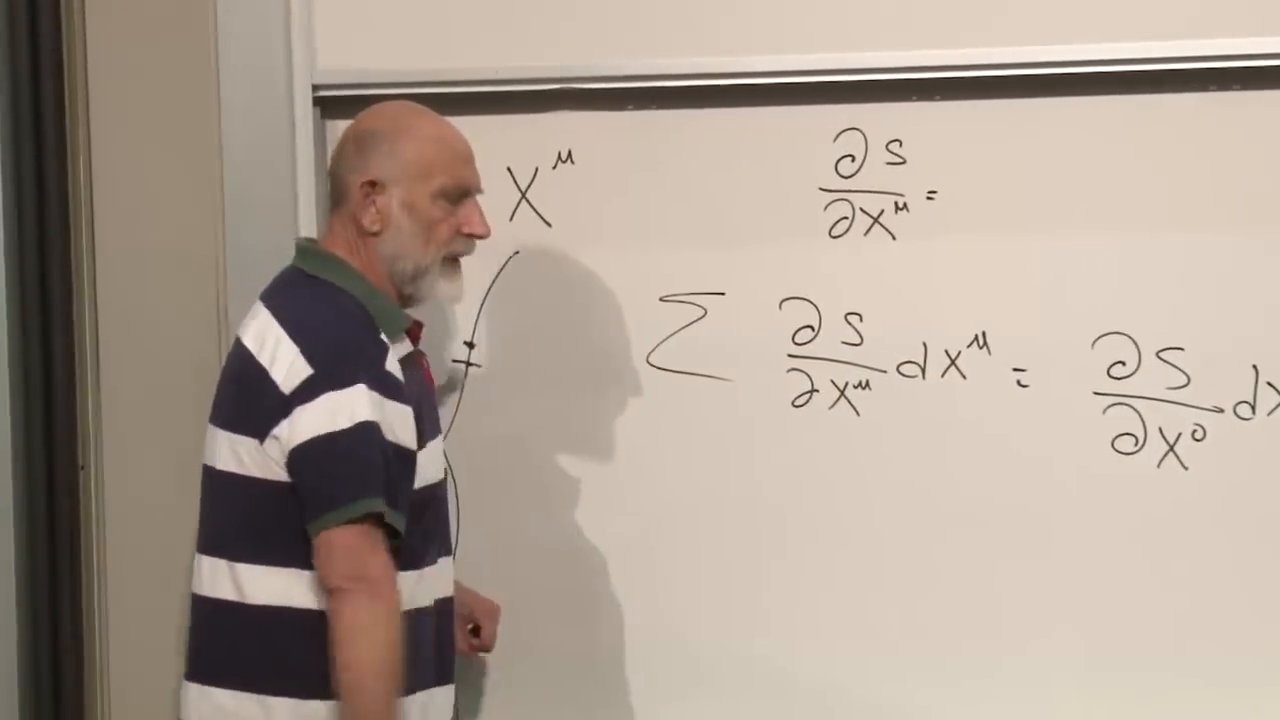
\includegraphics[width=0.90\textwidth]{lecture_07_figure_01.png}
\caption{下付き添字の勾配と上付き添字の変位から組み立てられたスカラー微分。}
\lectureframe{00:08:20}
\end{figure}

アインシュタインの規約は今や直ちに適用できる。すなわち、一度上付きで一度下付きで現れる添字は和を取る。したがって、
\eqref{eq:sr7-total-differential}における縮約はスカラーである。ベクトルと余ベクトルにはより深い幾何学的解釈があるが、その議論は一般相対論まで延期される。

\subsection{添字を上げる}

すべての四元ベクトルには、計量によって関係づけられた上付き形と下付き形がある：
\begin{equation}
A_\mu=\eta_{\mu\nu}A^\nu.
\end{equation}
\eqref{eq:sr7-metric}を用いると、
\begin{equation}
A_0=-A^0,
\qquad
A_m=A^m,
\qquad m=1,2,3.
\label{eq:sr7-lowering}
\end{equation}
したがって、添字を上げたり下げたりすると時間成分の符号が変わり、空間成分には何も起こらない。同じ規則が微分にも当てはまる：
\begin{equation}
\begin{aligned}
\partial_\mu
&=
\left(
\frac{\partial}{\partial t},
\frac{\partial}{\partial x},
\frac{\partial}{\partial y},
\frac{\partial}{\partial z}
\right),\\[0.5em]
\partial^\mu
&=
\left(
-\frac{\partial}{\partial t},
\frac{\partial}{\partial x},
\frac{\partial}{\partial y},
\frac{\partial}{\partial z}
\right).
\end{aligned}
\label{eq:sr7-raised-gradient}
\end{equation}

\begin{figure}[htbp]
\centering
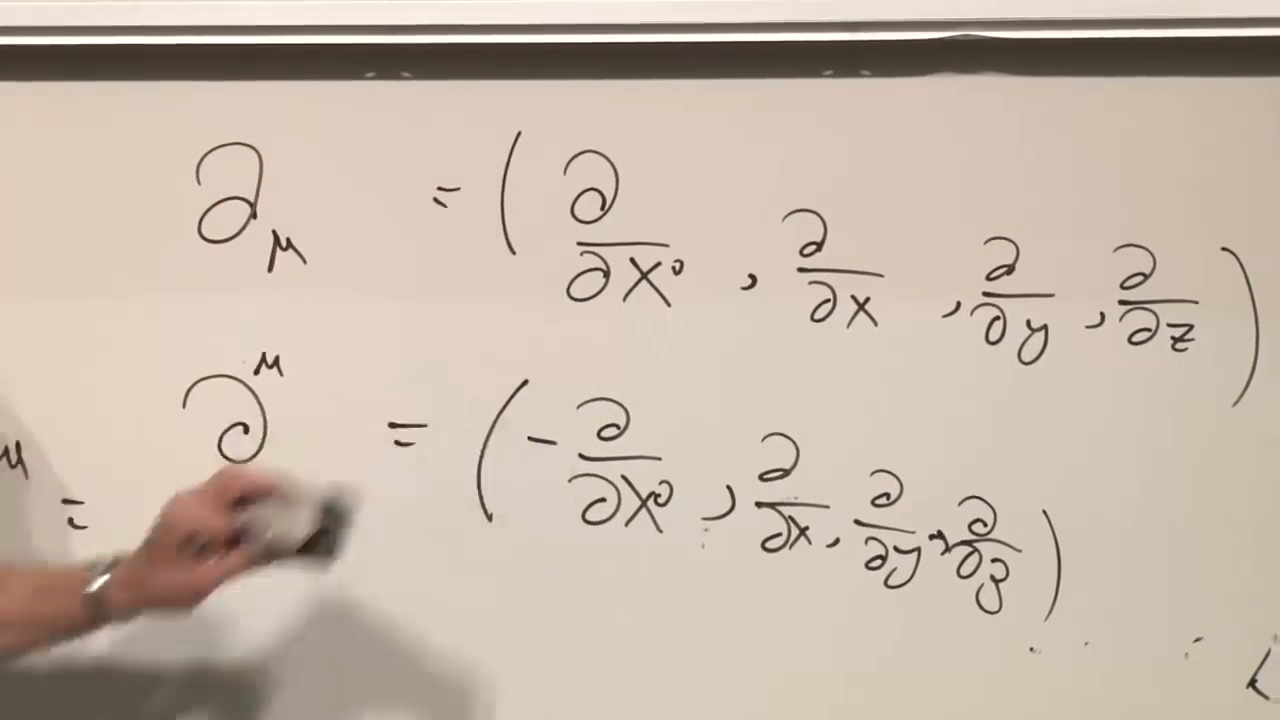
\includegraphics[width=0.90\textwidth]{lecture_07_figure_02.png}
\caption{下付きおよび上付き添字の微分演算子。時間成分だけが符号を変える。}
\lectureframe{00:12:30}
\end{figure}

\begin{classroomqa}
\audiencequestion{偏微分は常に下付き添字を持ちますか、またそれを上げることもできますか。}
\lecturerresponse{演算子\(\partial/\partial x^\mu\)は自然に
\(\partial_\mu\)、すなわち余ベクトルである。計量を適用すると
\(\partial^\mu=\eta^{\mu\nu}\partial_\nu\)が得られる。平坦時空では、これは単に時間成分を反転させる。\lecturetimestamp{00:11:00}}
\end{classroomqa}

不変間隔はおなじみの例である：
\begin{equation}
x_\mu x^\mu
=
x^2+y^2+z^2-t^2.
\label{eq:sr7-interval}
\end{equation}
一つの上付き添字と一つの下付き添字の縮約はローレンツスカラーを生む。この単純な認識規則こそ、この記法をこれほど注意深く扱う理由である。

\section{理論を構成するための四つの原理}

ある実験が新しい現象を明らかにし、その理論を定式化したいとしよう。四つの原理がその探求を組織する。それらは最終的には洗練を要するかもしれないが、現在成功している基礎理論はすべてこのパターンに当てはまる。

\subsection{作用原理}

第一の要請は作用である。粒子力学では、
\begin{equation}
I[x]
=
\int dt\,L(x,\dot x),
\label{eq:sr7-particle-action-general}
\end{equation}
であり、物理的な経路はその端点を固定する変分の下で停留である：
\begin{equation}
\delta I=0.
\end{equation}
そこから得られる方程式は
\begin{equation}
\frac{d}{dt}
\left(
\frac{\partial L}{\partial\dot x^m}
\right)
=
\frac{\partial L}{\partial x^m}.
\label{eq:sr7-EL}
\end{equation}
である。

作用原理は美的な装飾ではない。それは対称性と保存則を結びつける枠組みである。作用の時間並進対称性はエネルギー保存をもたらし、空間並進は運動量保存をもたらし、関連する対称性が他の保存量の基礎となる。作用それ自体が保存則なのではなく、対称性が保存則となる構造が作用なのである。

\subsection{局所性}

第二の要請は局所性である。バイオリン弦の一点が乱されれば、隣接する部分がまず応答する。その隣が次に応答し、乱れが伝播する。影響は最終的に弦全体に及ぶが、短時間における直接の影響は局所的である。

粒子に対しては、局所性は軌道に沿って評価されるラグランジアンによって表現される。それは同じ時刻における位置と速度に依存し、任意の遠く離れた時刻の対には依存しない。場\(\phi(x)\)に対しては、
\begin{equation}
I[\phi]
=
\int d^4x\,
\mathcal L\!\left(\phi,\partial_\mu\phi\right).
\label{eq:sr7-local-field-action}
\end{equation}
である。ある事象における密度は、その事象における場とその一階導関数に依存する。そこには、ここの場と無関係な遠方の点における場との直接の積は含まれない。

\begin{figure}[htbp]
\centering
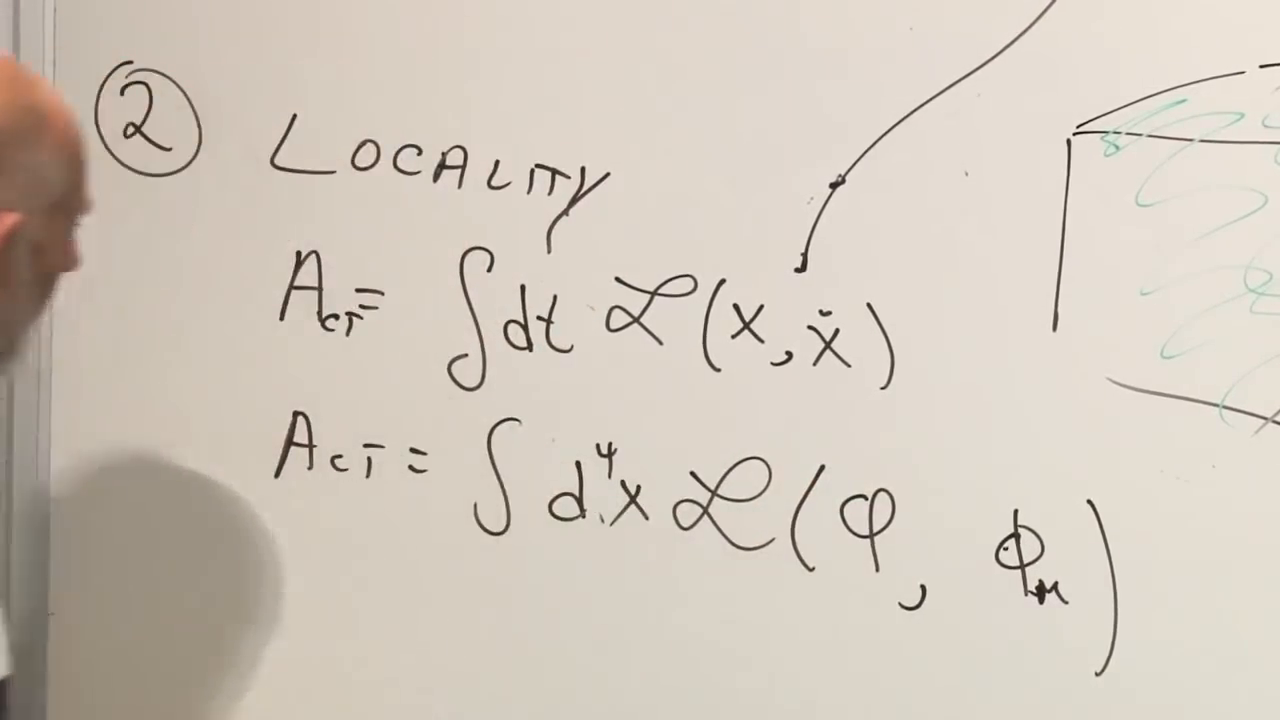
\includegraphics[width=0.90\textwidth]{lecture_07_figure_03.png}
\caption{局所性の原理の下に示された粒子と場の作用。}
\lectureframe{00:19:30}
\end{figure}

これが、局所的な運動方程式が微分方程式である理由である。導関数は無限小に隣接する値を比較する。非局所的な代替案は、現在の加速度をまったく異なる時刻の力に関係づけたり、二つの遠く離れた時刻の速度を第三の時刻の力に関係づけたりするかもしれない。そのような法則は数学的には想像可能であるが、局所性はそれらを排除する。

\begin{classroomqa}
\audiencequestion{量子もつれはこの局所性の原理と矛盾するのだろうか。}
\lecturerresponse{ここで用いられている力学的な意味では矛盾しない。もつれは相関を生み出すが、アリスによる局所的な操作を用いてボブの縮約状態を変えたり、彼に瞬時に制御可能な信号を送ったりすることはできない。ニッケル・アンド・ダイムの類推はその区別を際立たせる。一方のコインを見れば、相手がどの相関したコインを持っているかが分かるが、それは遠方のコインに作用するものではない。量子相関はその古典的な類推よりも豊かであるが、それでも超光速の信号伝達を与えるものではない。\lecturetimestamp{00:20:02}}
\end{classroomqa}

\subsection{ローレンツ不変性}

第三の要請は、法則がすべての慣性系で同じ形をとることである。実用的な構成規則は単純である。ラグランジアンはローレンツスカラーでなければならず、それゆえ作用は不変である。\(\partial_\mu\phi\,\partial^\mu\phi\)のような上--下の縮約が構成要素を与える。

一般相対性理論ではこの言明は拡張される。被積分関数はスカラー密度であり、不変性はローレンツ変換から任意の座標変換へと拡張される。その洗練は現在の原理を置き換えるものではなく、その曲がった時空における形である。

\begin{classroomqa}
\audiencequestion{ローレンツ不変性は真に一般的な原理ではなく、特殊相対性理論のための規則にすぎないのだろうか。}
\lecturerresponse{平坦な時空における非重力問題に対しては、ローレンツ不変性が正しい言明である。曲がった時空では、スカラーラグランジアンを適切なスカラー密度に置き換え、任意の座標変換の下での不変性を要求する。その洗練を除けば、同じ構成の哲学が生き残る。\lecturetimestamp{00:24:16}}
\end{classroomqa}

\begin{classroomqa}
\audiencequestion{粒子ラグランジアンと場のラグランジアン密度の次元は何か。}
\lecturerresponse{粒子ラグランジアンはエネルギーの次元をもつ。\(I=\int dt\,d^3x\,\mathcal L\)では、空間的な測度が体積を与えるので、\(\mathcal L\)は単位体積あたりのエネルギーの次元をもつ。それを空間にわたって積分すると、エネルギーの次元をもつ通常のラグランジアンが得られる。\lecturetimestamp{00:25:49}}
\end{classroomqa}

\subsection{ゲージ不変性}

第四の要請はゲージ不変性である。この時点では、それは意図的に謎のままにされている。聴衆の一人が有用な予想を述べる。おそらく、物理を変えずにラグランジアンに特定のものを加えることができるのではないか。それは近いが、「特定の」という言葉がほぼすべての仕事をすることになる。

\begin{figure}[htbp]
\centering
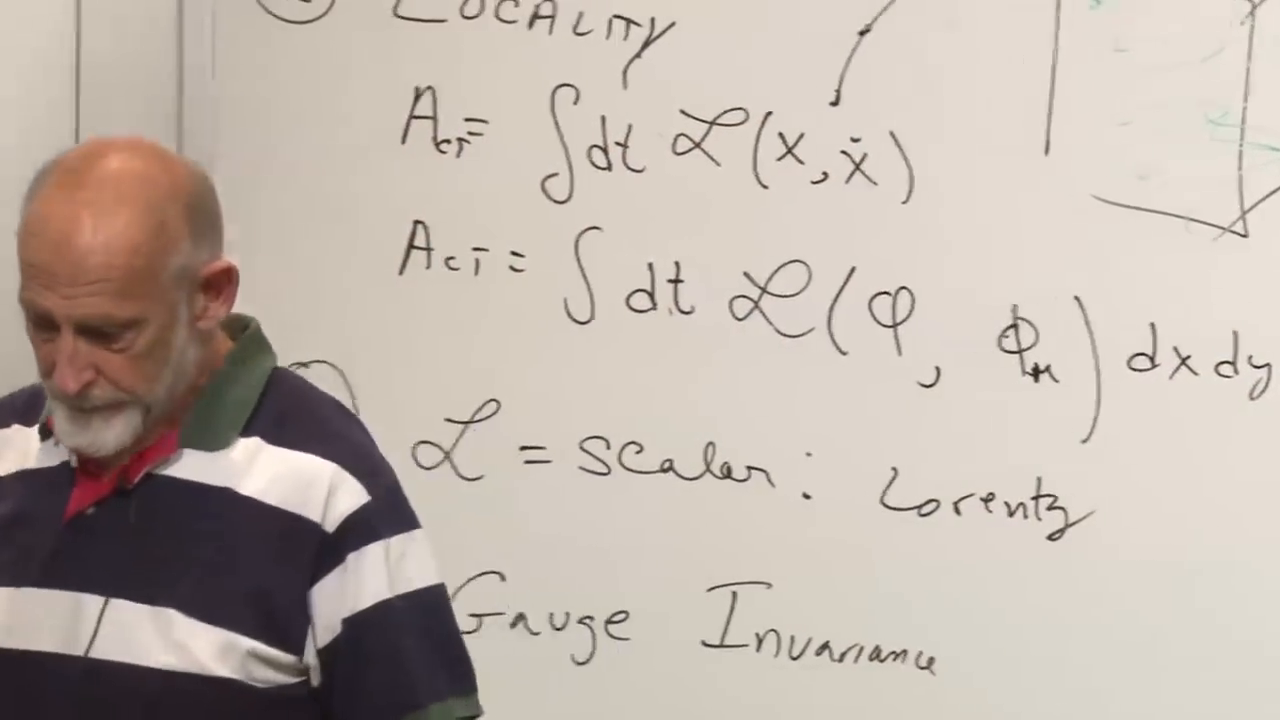
\includegraphics[width=0.90\textwidth]{lecture_07_figure_04.png}
\caption{局所性、スカラー構成、ローレンツ不変性、ゲージ不変性が黒板にまとめられた。}
\lectureframe{00:27:00}
\end{figure}

電荷を持つ粒子の計算にすでに含まれているので、定義は後回しにする。その計算を繰り返すのは回り道ではない。それは、なぜベクトルポテンシャルが我々に押し付けられるのか、そしてひとたび導入されればなぜそれが冗長性を含むのかを明らかにするであろう。

\section{なぜベクトルポテンシャルが必要なのか}

ゆっくり運動する荷電粒子に対して、目標となる方程式はおなじみのローレンツ力の法則
\begin{equation}
m\mathbf a
=
e\left(
\mathbf E+\mathbf v\times\mathbf B
\right).
\label{eq:sr7-lorentz-target}
\end{equation}

\begin{figure}[htbp]
\centering
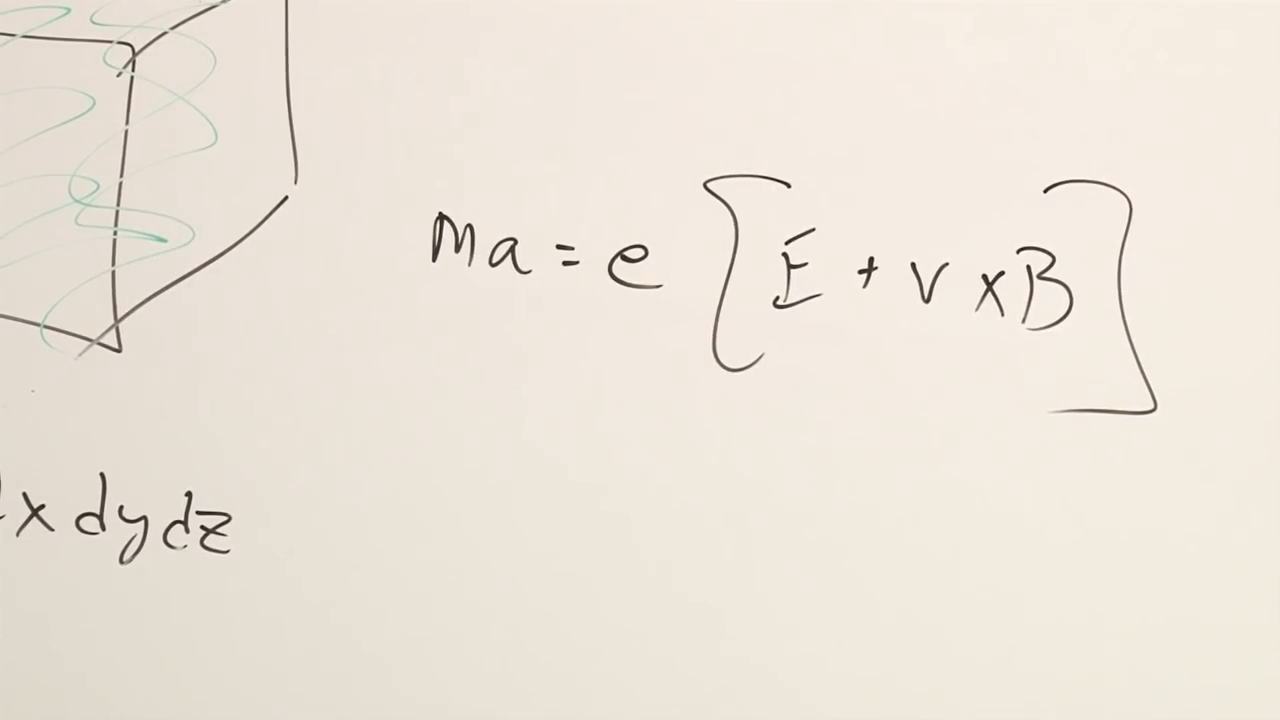
\includegraphics[width=0.90\textwidth]{lecture_07_figure_05.png}
\caption{ベクトルポテンシャルが再導入される前に書かれた、おなじみの力の法則。}
\lectureframe{00:29:08.870}
\end{figure}

\eqref{eq:sr7-lorentz-target}にはベクトルポテンシャルは現れない。運動方程式は\(\mathbf E\)と\(\mathbf B\)で直接書くことができる。困難はより構造的なものである。講義で用いられた局所性とローレンツ不変性の仮定の下では、荷電粒子の相互作用は、それらの場、位置、速度だけを用いて世界線作用として直接書くことはできない。局所的なスカラー結合を構成するにはポテンシャル\(A_\mu\)が必要である。

\begin{classroomqa}
\audiencequestion{力の法則がすでに\(\mathbf E\)と\(\mathbf B\)だけを含んでいるのなら、なぜ\(A_\mu\)を導入するのか。}
\lecturerresponse{運動方程式はまだ作用原理ではないからである。この講義の局所ローレンツ不変な枠組みの中では、荷電粒子の作用には四元ポテンシャルが必要である。場だけでも力を述べることはできるが、力をスカラー世界線作用から導出することを可能にする対象はポテンシャルである。\lecturetimestamp{00:29:06}}
\end{classroomqa}

\subsection{世界線作用}

候補となる作用は自由部分と相互作用部分を持つ。
\begin{equation}
I[x]
=
-m\int d\tau
-e\int A_\mu(x)\,dx^\mu.
\label{eq:sr7-worldline-action}
\end{equation}
第一項は軌道の各無限小線分の固有時長さを加え合わせる。それは構成上スカラーである。第二項では、\(A_\mu(x)\)が粒子の占める事象で評価され、変位\(dx^\mu\)と縮約される。その増分もまたスカラーであり、世界線に沿って局所的である。

\begin{figure}[htbp]
\centering
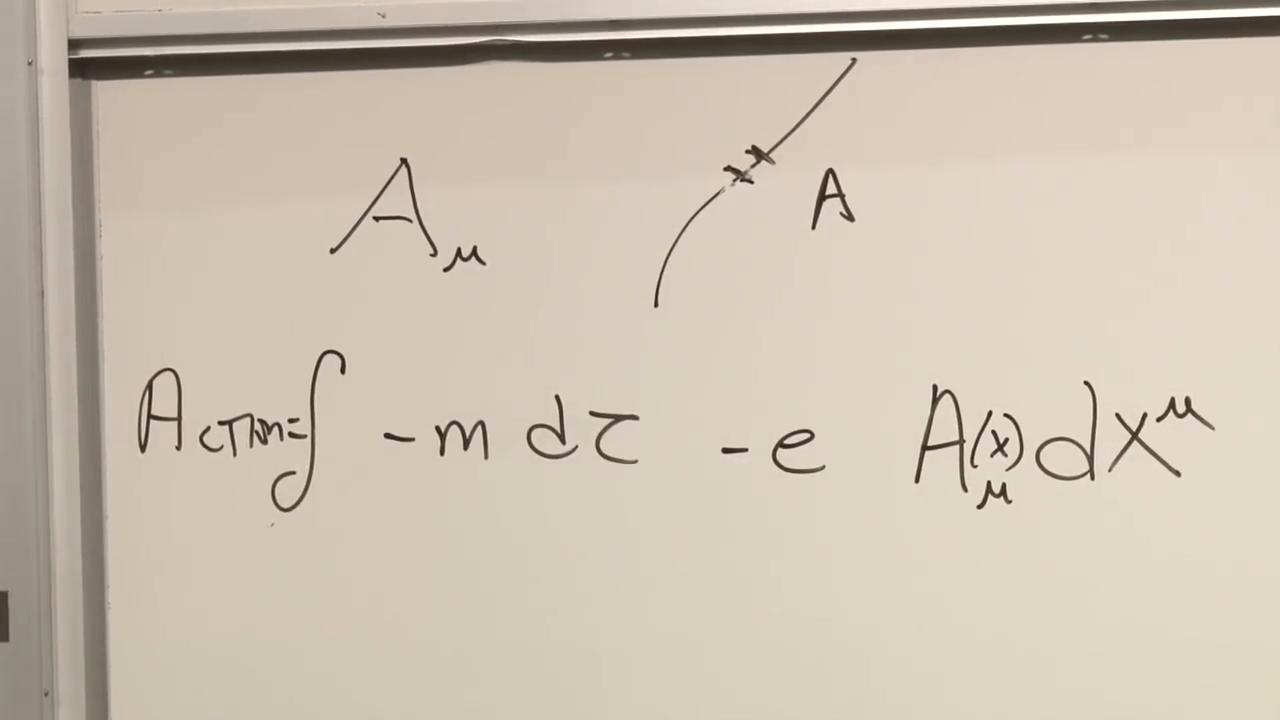
\includegraphics[width=0.90\textwidth]{lecture_07_figure_06.png}
\caption{荷電粒子作用の二つの部分と局所的な縮約\(A_\mu(x)dx^\mu\)。}
\lectureframe{00:31:20}
\end{figure}

\subsection{作用を通常の時間で書き直す}

おなじみのオイラー--ラグランジュ方程式を用いるために、各世界線増分を\(dt\)で割る。
\begin{equation}
\frac{d\tau}{dt}
=
\sqrt{1-\dot{\mathbf x}^{\,2}},
\qquad
\dot{\mathbf x}^{\,2}
=
\dot x^2+\dot y^2+\dot z^2.
\end{equation}
\(dx^\mu/dt\)の四つの成分は
\begin{equation}
\frac{dx^\mu}{dt}
=
\left(1,\dot x,\dot y,\dot z\right).
\end{equation}
したがって、
\begin{align}
I
&=
\int dt\,
\left[
-m\sqrt{1-\dot{\mathbf x}^{\,2}}
-eA_\mu\frac{dx^\mu}{dt}
\right]
\notag\\
&=
\int dt\,
\left[
-m\sqrt{1-\dot{\mathbf x}^{\,2}}
-e\left(A_0+A_m\dot x^m\right)
\right].
\label{eq:sr7-action-in-t}
\end{align}
通常時間のラグランジアンはしたがって
\begin{equation}
\begin{aligned}
L(x,\dot x,t)
&=
-m\sqrt{1-\dot{\mathbf x}^{\,2}}
\\
&\quad -e\left[
A_0(x,t)+A_m(x,t)\dot x^m
\right].
\end{aligned}
\label{eq:sr7-lagrangian}
\end{equation}

\begin{figure}[htbp]
\centering
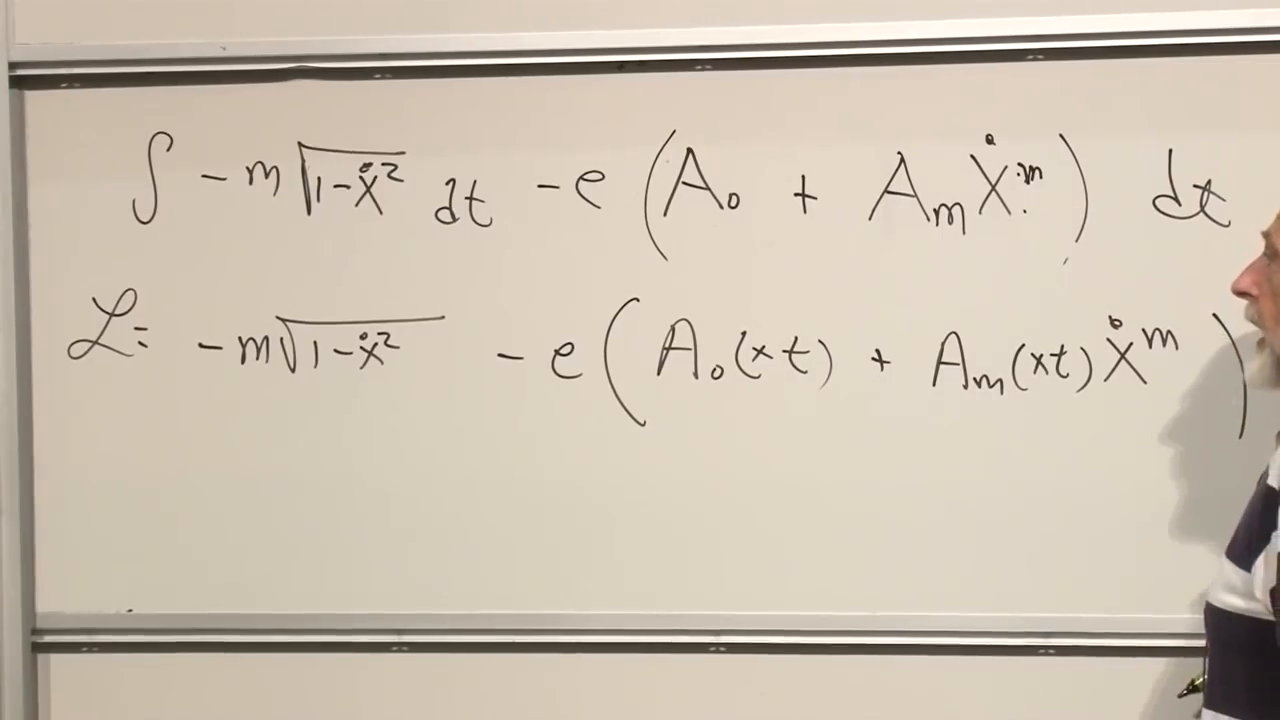
\includegraphics[width=0.90\textwidth]{lecture_07_figure_07.png}
\caption{通常時間の積分として書き直された世界線作用と、その被積分関数から読み取られるラグランジアン。}
\lectureframe{00:35:30}
\end{figure}

この段階で想像の部分は終わりである。ひとたびラグランジアンが選ばれれば、あとは機械的である。その機械的操作は長く退屈なものになり得るが、その退屈さは空虚ではない。電気的、磁気的、相対論的構造を明らかにするのはそれだからである。講師は、原理を発見することが楽しい部分であり、そのすべての帰結を導出することは大学院生に与えるものである、と冗談を言う。

\begin{classroomqa}
\audiencequestion{この計算で\(A_m\)や\(\dot x^m\)の空間添字を上付きまたは下付きに動かしてもよいか。}
\lecturerresponse{はい。空間計量は単位行列なので、ラテン添字を上げ下げしてもその成分の値は変わらない。符号に注意を要するのは時間添字である。\lecturetimestamp{00:34:10}}
\end{classroomqa}

\section{オイラー--ラグランジュ計算}

\subsection{正準運動量とライブな訂正}

一つの空間成分\(x^m\)を選ぶ。\eqref{eq:sr7-lagrangian}の自由項を微分すると
\begin{equation}
\frac{m\dot x_m}{\sqrt{1-\dot{\mathbf x}^{\,2}}}
=
m u_m,
\qquad
u^\mu\equiv\frac{dx^\mu}{d\tau}.
\end{equation}
最初の板書の試みはそこで止まる。聴衆からの訂正がその抜けを捉える。相互作用項もまた\(\dot x^m\)に依存する。完全な導関数は
\begin{equation}
\frac{\partial L}{\partial\dot x^m}
=
\frac{m\dot x_m}{\sqrt{1-\dot{\mathbf x}^{\,2}}}
-eA_m
=
m u_m-eA_m.
\label{eq:sr7-canonical-momentum}
\end{equation}

\begin{classroomqa}
\audiencequestion{\(\partial L/\partial\dot x^m\)の最初の表式は電磁項からの寄与を欠いているのではないか。}
\lecturerresponse{はい。
\(-eA_n\dot x^n\)を\(\dot x^m\)に関して微分すると
\(-eA_m\)が寄与する。訂正された正準運動量は
\(m u_m-eA_m\)であり、力学的運動量だけではない。
\lecturetimestamp{00:37:24}}
\end{classroomqa}

\begin{figure}[htbp]
\centering
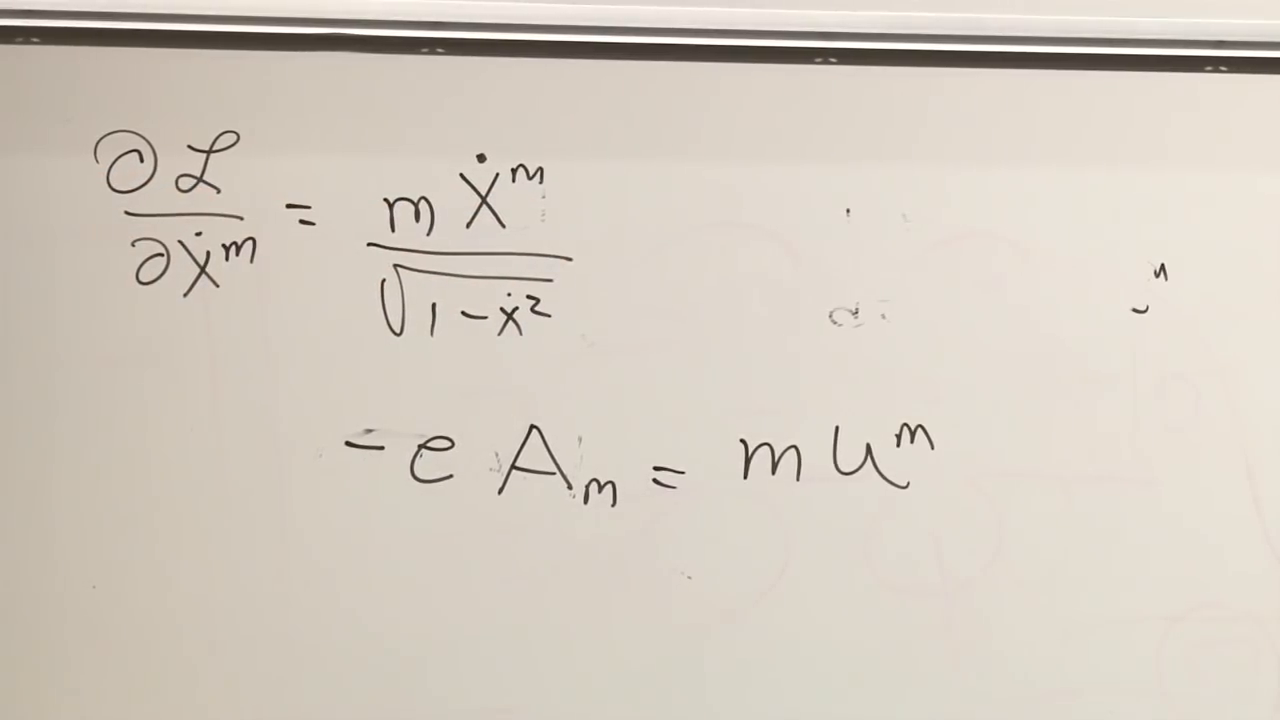
\includegraphics[width=0.90\textwidth]{lecture_07_figure_08.png}
\caption{力学的項とポテンシャル項の両方を持つ、訂正された正準運動量。}
\lectureframe{00:38:30}
\end{figure}

\subsection{運動する経路に沿って微分する}

オイラー--ラグランジュ方程式の左辺は
\begin{equation}
\frac{d}{dt}
\left(
\frac{\partial L}{\partial\dot x^m}
\right)
=
m\frac{du_m}{dt}
-e\frac{dA_m(x(t),t)}{dt}.
\end{equation}
ポテンシャルは二つの理由で変化する。すなわち、時間に陽に依存し得ること、そして粒子がその空間的変化の中を運動することである。連鎖律により
\begin{equation}
\frac{dA_m}{dt}
=
\partial_0A_m
+\dot x^n\partial_nA_m.
\label{eq:sr7-chain-rule}
\end{equation}
長々と書けば、第二項は
\begin{equation}
\dot x\,\frac{\partial A_m}{\partial x}
+\dot y\,\frac{\partial A_m}{\partial y}
+\dot z\,\frac{\partial A_m}{\partial z}.
\end{equation}

\begin{figure}[htbp]
\centering
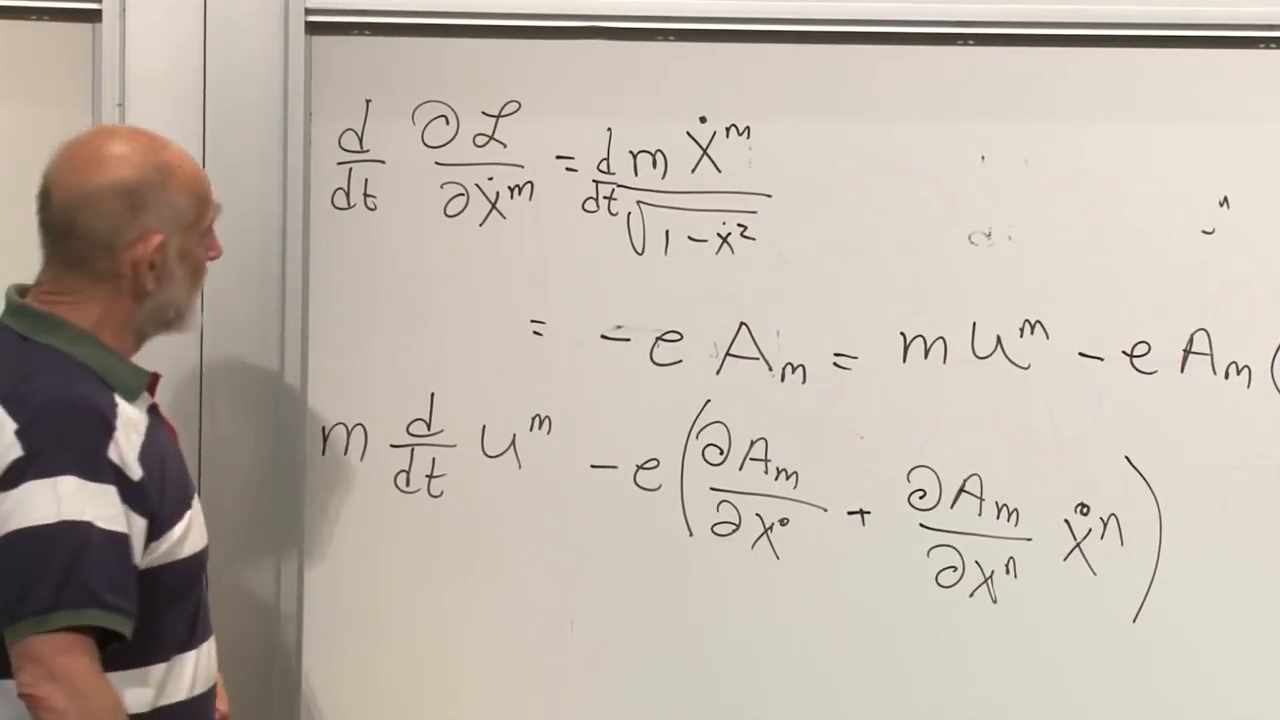
\includegraphics[width=0.90\textwidth]{lecture_07_figure_09.png}
\caption{\(A_m\)の時間導関数の陽的部分と移流的部分。}
\lectureframe{00:42:10}
\end{figure}

右辺では、
\begin{equation}
\frac{\partial L}{\partial x^m}
=
-e\partial_mA_0
-e\dot x^n\partial_mA_n.
\label{eq:sr7-spatial-derivative-L}
\end{equation}
自由項には明示的な位置依存性がない。\eqref{eq:sr7-spatial-derivative-L}において、\(m\)は1つの方程式を選び出す自由添字であり、\(n\)は繰り返されるダミー添字であって和が取られる。そのダミー添字の名前を変えても何も変わらない。この区別があるため、講師は項をまとめる前に文字について立ち止まって確認するのである。

両辺を等置して整理すると、
\begin{equation}
m\frac{du_m}{dt}
=
e\left(
\partial_0A_m-\partial_mA_0
\right)
+e\dot x^n
\left(
\partial_nA_m-\partial_mA_n
\right).
\label{eq:sr7-grouped-force}
\end{equation}
が得られる。

\begin{figure}[htbp]
\centering
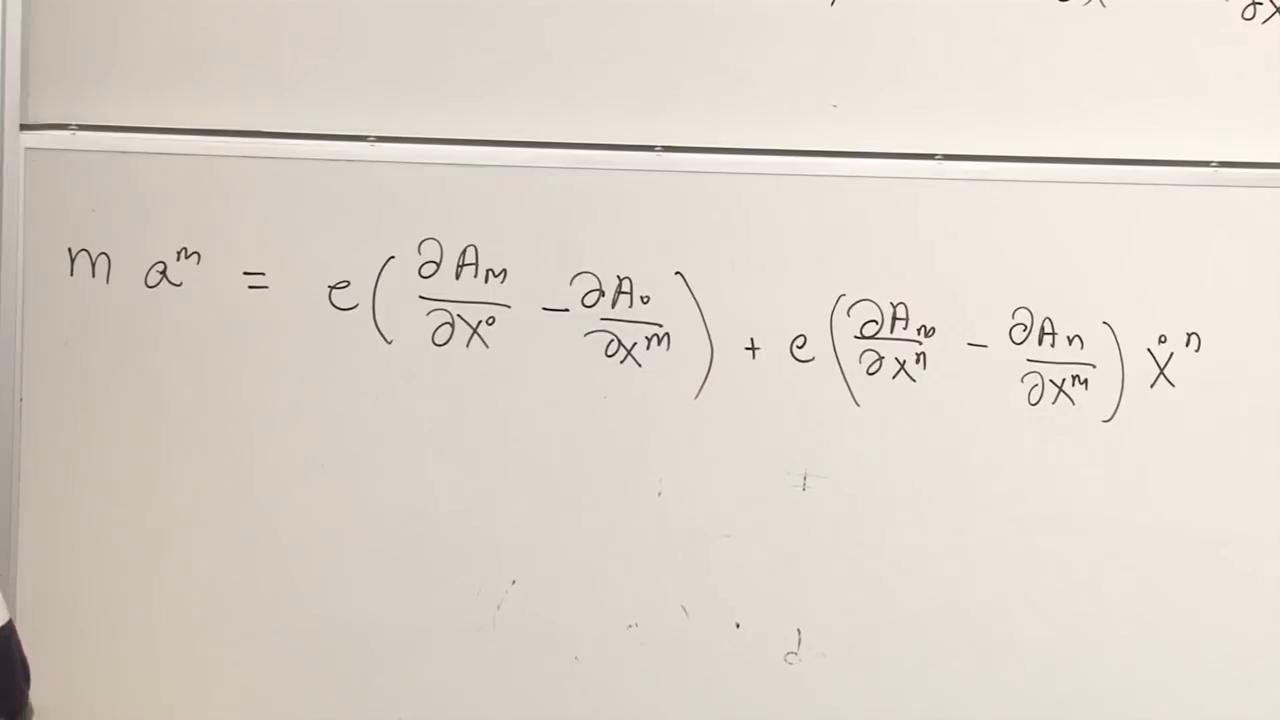
\includegraphics[width=0.90\textwidth]{lecture_07_figure_10.png}
\caption{力は、速度に依存しない括弧と、速度に線形な反対称括弧に分離された。}
\lectureframe{00:49:30}
\end{figure}

\subsection{電場と磁場の認識}

最初の括弧には粒子の速度が含まれていない。この作用の規約では、
\begin{equation}
E_m
\equiv
\partial_0A_m-\partial_mA_0.
\label{eq:sr7-E-from-A}
\end{equation}
と定義する。これはまさに電場の操作的役割を担っている。2番目の括弧は空間添字について反対称である：
\begin{equation}
C_{mn}
\equiv
\partial_nA_m-\partial_mA_n.
\label{eq:sr7-C}
\end{equation}
その3つの独立な成分は空間的ポテンシャルの回転であり、講義の規約で向きを選ぶと
\begin{equation}
\dot x^n C_{mn}
=
\left(\mathbf v\times\mathbf B\right)_m.
\label{eq:sr7-magnetic-identification}
\end{equation}
となる。成分ごとの詳細な確認は黒板での演習問題として残される。構造的な同定はすでに見えている：ベクトルの反対称な空間微分は3つの成分をもち、それは\(\mathbf B\)が担う成分の数にちょうど等しく、それが速度に掛かっている。

\begin{figure}[htbp]
\centering
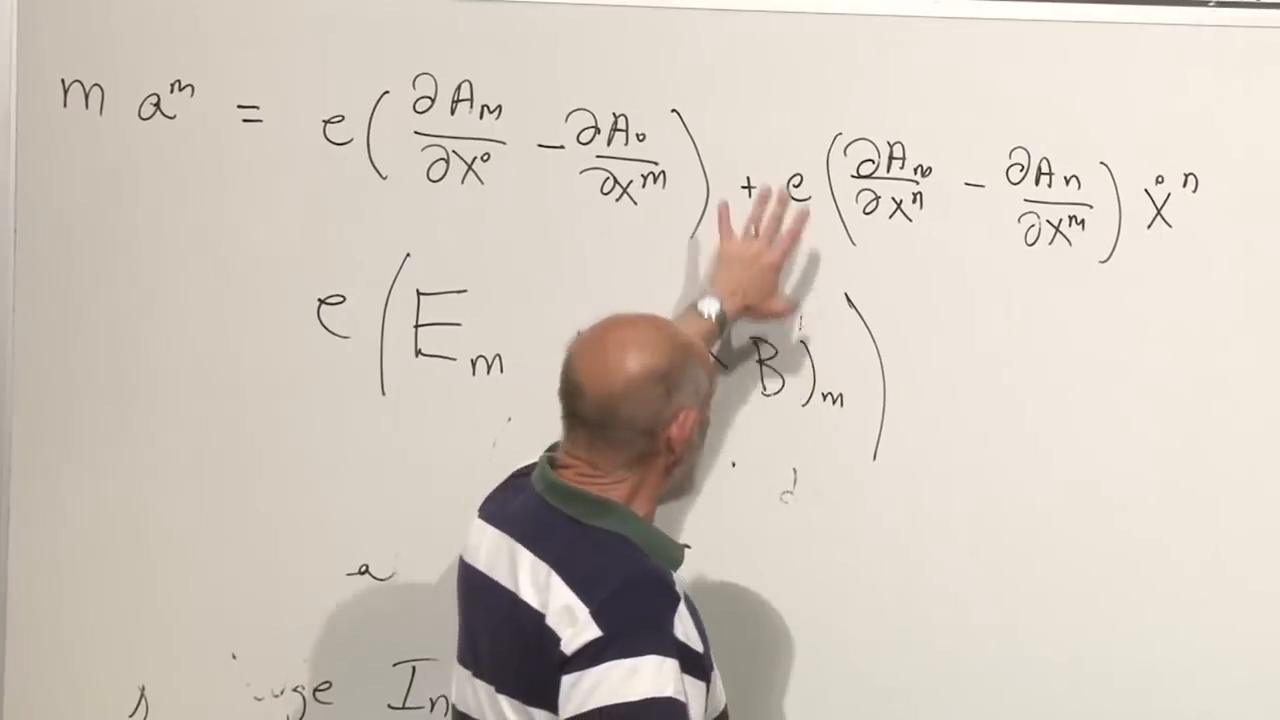
\includegraphics[width=0.90\textwidth]{lecture_07_figure_11.png}
\caption{2つの微分括弧がローレンツ力の電場部分と磁場部分として同定された。}
\lectureframe{00:52:00}
\end{figure}

したがって式\eqref{eq:sr7-grouped-force}は、ベクトルポテンシャルの作用からローレンツ力を再現したことになる。さらに重要なことも成し遂げている：後に場のテンソルとなる反対称化された微分を露わにしたのである。

\section{通常の時間から四元ベクトル方程式へ}

\subsection{固有時間への変換}

\eqref{eq:sr7-grouped-force}の左辺はニュートン的な加速度\(d\mathbf v/dt\)ではない。それは四元速度成分の通常時間に関する微分である：
\begin{equation}
\frac{du^m}{dt}
=
\frac{du^m}{d\tau}\frac{d\tau}{dt}.
\end{equation}
方程式に\(dt/d\tau\)を掛ける。すると
\begin{equation}
\dot x^n\frac{dt}{d\tau}
=
\frac{dx^n}{dt}\frac{dt}{d\tau}
=
u^n,
\qquad
\frac{dt}{d\tau}=u^0.
\end{equation}
空間的方程式は
\begin{align}
m\frac{du^m}{d\tau}
&=
e\left(
\partial_0A_m-\partial_mA_0
\right)u^0
\notag\\
&\quad
+e\left(
\partial_nA_m-\partial_mA_n
\right)u^n.
\label{eq:sr7-proper-spatial}
\end{align}
となる。

\begin{figure}[htbp]
\centering
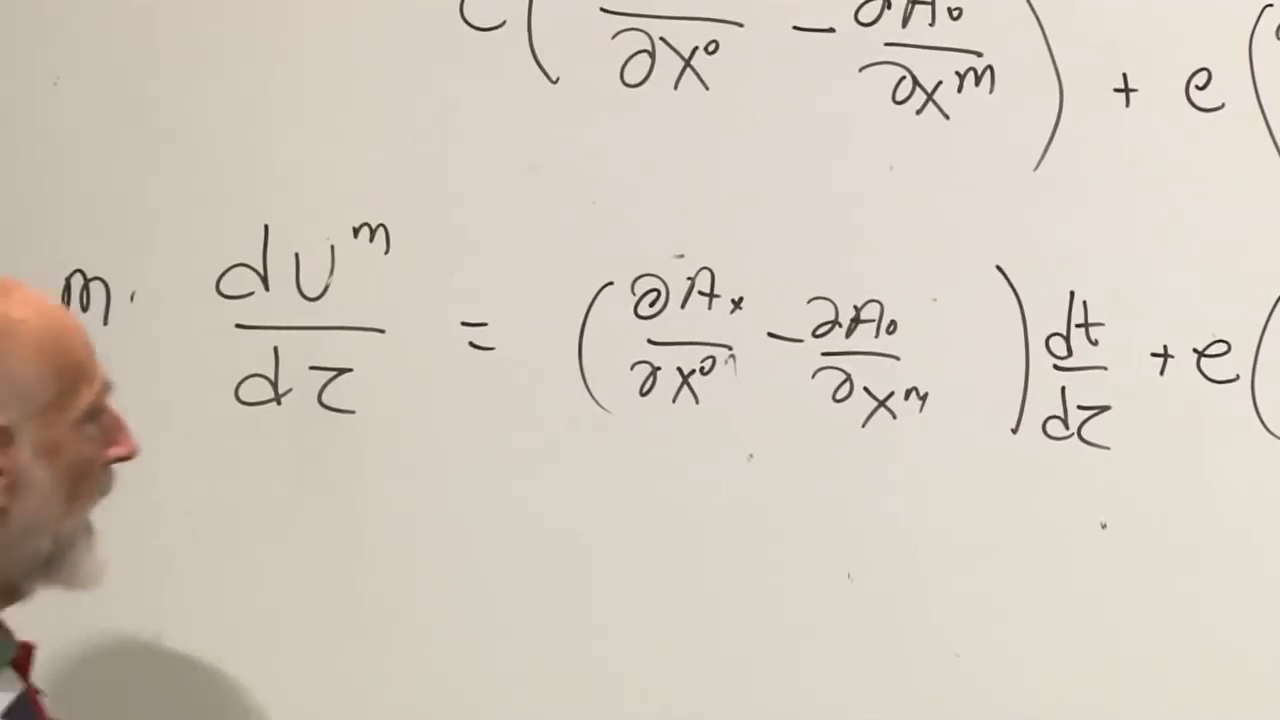
\includegraphics[width=0.90\textwidth]{lecture_07_figure_12.png}
\caption{因子\(dt/d\tau\)は通常の速度を四元速度の成分に変換する。}
\lectureframe{00:56:30}
\end{figure}

左辺は固有加速度である：
\begin{equation}
\frac{du^\mu}{d\tau}
=
\frac{d^2x^\mu}{d\tau^2}.
\end{equation}
これは四元ベクトルである。したがって右辺は、\(u^\nu\)に作用する2階のテンソルから組み立てられなければならない。

\subsection{場のテンソルと力の法則}

規約として
\begin{equation}
F_{\mu\nu}
\equiv
\partial_\mu A_\nu-\partial_\nu A_\mu.
\label{eq:sr7-F-definition}
\end{equation}
を選ぶ。これは反対称である：
\begin{equation}
F_{\mu\nu}=-F_{\nu\mu}.
\end{equation}
\eqref{eq:sr7-worldline-action}における相互作用の符号を用いると、コンパクトな方程式は
\begin{equation}
\boxed{
m\frac{du^\mu}{d\tau}
=
-eF^\mu{}_\nu u^\nu
}.
\label{eq:sr7-covariant-force}
\end{equation}
となる。等価に、\(F_{\mu\nu}\)と名付ける前には、
\begin{equation}
m\frac{du^\mu}{d\tau}
=
e\left(
\partial_\nu A^\mu-\partial^\mu A_\nu
\right)u^\nu.
\end{equation}
である。計量、電荷、ポテンシャルの規約が異なれば、全体の符号は再分配される。不変な内容は、ポテンシャルの反対称化された微分と、その四元速度との縮約である。

\begin{figure}[htbp]
\centering
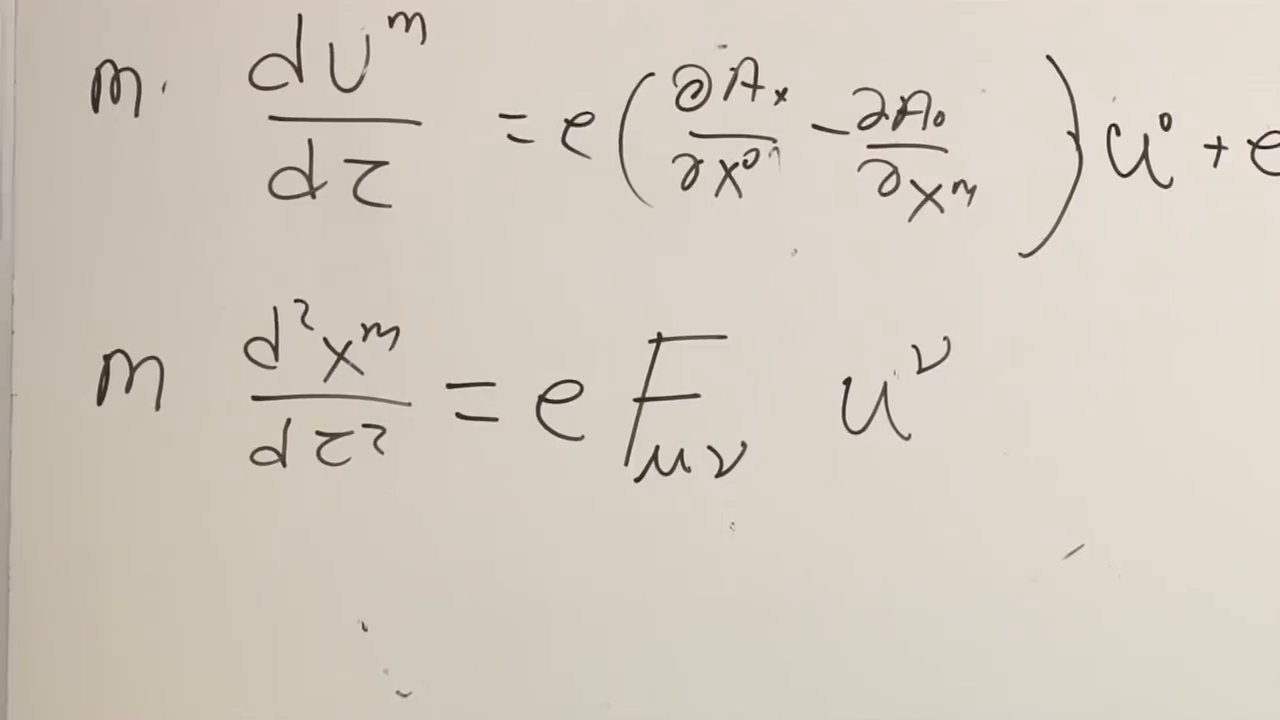
\includegraphics[width=0.90\textwidth]{lecture_07_figure_13.png}
\caption{固有時間の方程式が、四元速度に作用する2階の場のテンソルとしてまとめられた。}
\lectureframe{00:58:25}
\end{figure}

\begin{classroomqa}
\audiencequestion{この導出では3つの空間的方程式が得られた。なぜ4番目の方程式を付け加えることが許されるのか。}
\lecturerresponse{スカラー作用はローレンツ共変な結果を保証する。両辺の差が四元ベクトルであると認識されれば、ローレンツ変換はその空間成分と時間成分を混ぜ合わせる。四元ベクトル方程式が3つの成分だけをもつことは首尾一貫してはありえず、時間成分が空間成分に伴う。\lecturetimestamp{00:59:40}}
\end{classroomqa}

\begin{classroomqa}
\audiencequestion{\((1,2,3,4)\)のような数の固定されたリストそれ自体は、ローレンツ不変な四元ベクトルなのか。}
\lecturerresponse{いいえ。そのような数は、1つの選ばれた座標系におけるベクトルの成分でありうるが、成分は変換する。2次元であっても、成分\((1,2)\)をもつベクトルは、回転した座標系では\((0,\sqrt5)\)と記述できる。幾何学的なベクトルは持続するが、その数値的な成分のリストは持続しない。\lecturetimestamp{01:00:28}}
\end{classroomqa}

\begin{figure}[htbp]
\centering
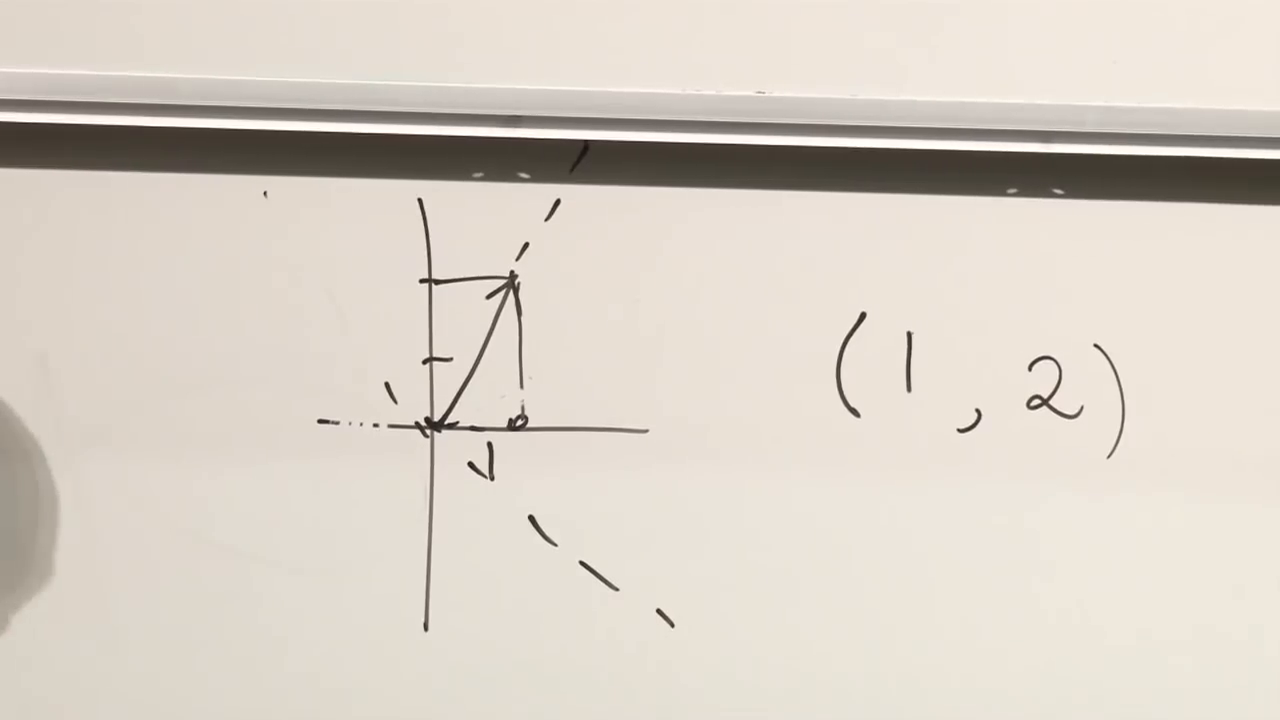
\includegraphics[width=0.90\textwidth]{lecture_07_figure_14.png}
\caption{2成分ベクトルが、そのベクトル自身に沿った軸で再表現されたもの。}
\lectureframe{01:02:00}
\end{figure}

\begin{classroomqa}
\audiencequestion{目的が通常の時間を固有時間で置き換えることであったなら、なぜ\(\partial_0A_m=\partial A_m/\partial t\)が依然として現れるのか。}
\lecturerresponse{目的はすべての文字\(t\)を消し去ることではなかった。力学を明白な四元ベクトル記法で書くことであった。演算子\(\partial_0\)は共変四元勾配の時間成分であり、ちょうど\(\partial_m\)がその空間成分であるのと同じである。それは四次元テンソルの内部に属している。\lecturetimestamp{01:05:10}}
\end{classroomqa}

講義はこの瞬間を用いて局所性を再確認する。局所的な方程式は、ある事象における加速度をその事象における場と速度に関係づける。それは現在の加速度を遠方の時刻における力に結びつけるものではない。

\begin{figure}[htbp]
\centering
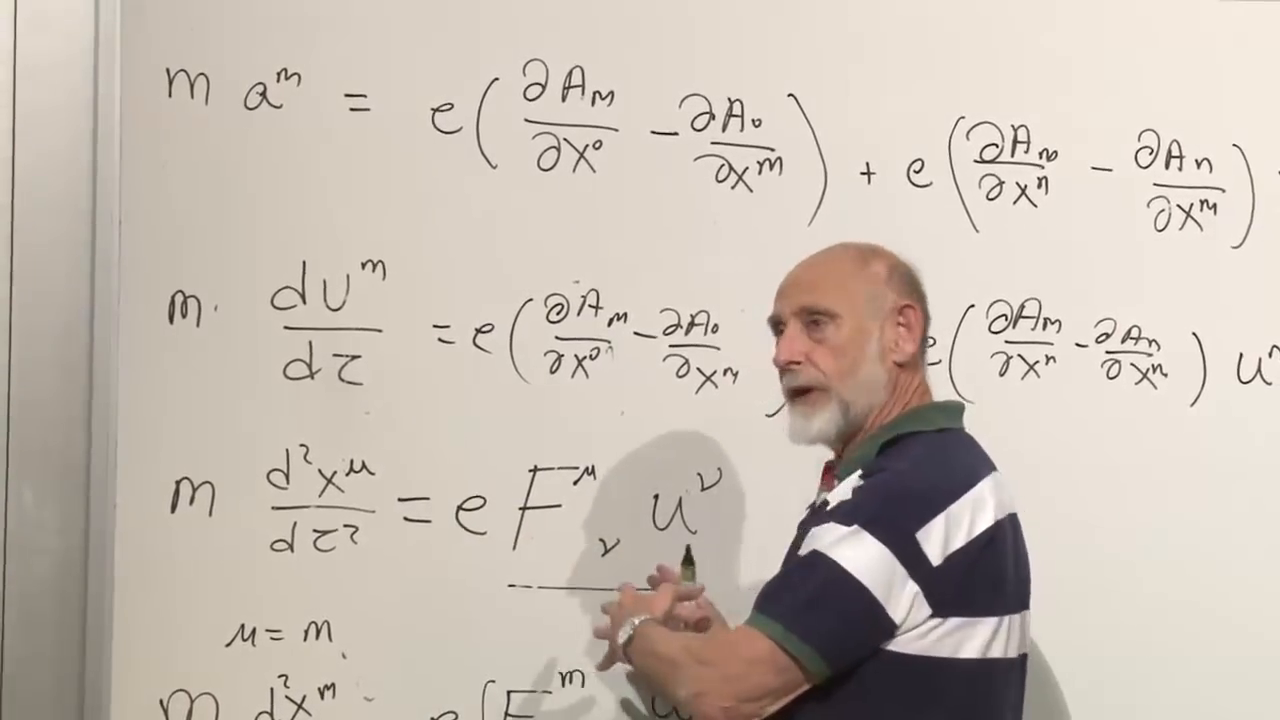
\includegraphics[width=0.90\textwidth]{lecture_07_figure_15.png}
\caption{局所性を微分力学として言い換えるために用いられた共変的な力の方程式。}
\lectureframe{01:05:50}
\end{figure}

\subsection{電磁場の成分を表示する}

すべて上付きのテンソルに対して、黒板で用いられた規約は次を与える。
\begin{equation}
F^{\mu\nu}
=
\begin{pmatrix}
0&-E_x&-E_y&-E_z\\
E_x&0&B_z&-B_y\\
E_y&-B_z&0&B_x\\
E_z&B_y&-B_x&0
\end{pmatrix}.
\label{eq:sr7-F-matrix}
\end{equation}
行の添字は\(\mu\)であり、列の添字は\(\nu\)である。混合された時間--空間の成分は電場を含み、空間--空間のブロックは磁場を含む。反対称性により対角成分はゼロに定まり、表示された十六個の成分は六個の独立な成分に減る。

\begin{figure}[htbp]
\centering
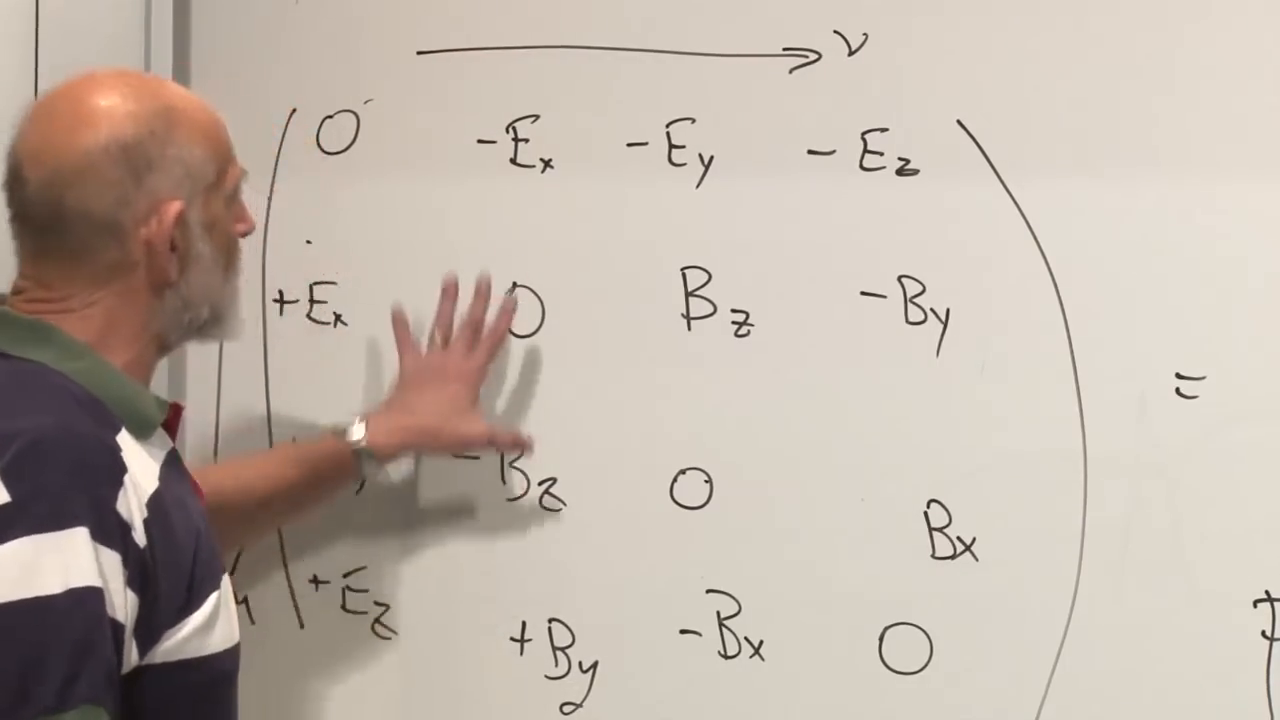
\includegraphics[width=0.90\textwidth]{lecture_07_figure_16.png}
\caption{完成した電磁テンソル。時間--空間の位置に電場の成分が、空間ブロックに磁場の成分が入る。}
\lectureframe{01:12:10}
\end{figure}

\begin{classroomqa}
\audiencequestion{どのテンソル添字が行を表し、どの添字が列を表すかを決める標準的な規則はありますか。}
\lecturerresponse{それは表示上の規約である。ここでは第一の添字
\(\mu\) が縦に走り、第二の添字 \(\nu\) が横に走る。
ひとたびその規約を宣言すれば、すべての成分は曖昧さなく読める。時間添字を上げると符号が導入されるが、行--列の規約は変わらない。\lecturetimestamp{01:09:01}}
\end{classroomqa}

\begin{classroomqa}
\audiencequestion{どの添字配置が反対称性を保つのか。}
\lecturerresponse{テンソル\(F_{\mu\nu}\)と\(F^{\mu\nu}\)は反対称である。混合配列\(F^\mu{}_\nu\)は通常の行列転置の下では反対称ではない。一方の時間添字を上げると電場の位置が変わり、時間--空間の対が対称になる一方、純粋に空間的な磁場ブロックは反対称のままである。講師は黒板で反対の可能性を簡単に検討して退けた後、この結論に達する。
\lecturetimestamp{01:13:18}}
\end{classroomqa}

\section{何が不変性と見なされるか}

ここで初めて第四の原理に戻る。不変性とは運動方程式を変えない変化である。作用それ自体は厳密に不変のままであってもよいし、変分方程式に影響を与えない境界項だけ変化してもよい。

\subsection{質量のないスカラーの定数シフト}

一次元空間における質量のないスカラー方程式を考える。
\begin{equation}
\frac{\partial^2\phi}{\partial t^2}
-\frac{\partial^2\phi}{\partial x^2}
=0,
\label{eq:sr7-wave}
\end{equation}
これは次から得られる。
\begin{equation}
\mathcal L_0
=
-\frac12\partial_\mu\phi\,\partial^\mu\phi.
\label{eq:sr7-massless-L}
\end{equation}
\(\phi\)が解ならば、
\begin{equation}
\phi\longrightarrow\phi+c,
\label{eq:sr7-constant-shift}
\end{equation}
も解である。ここで\(c\)は定数である。\(c\)のすべての導関数は消えるので、方程式も導関数のみのラグランジアンも変化しない。

\begin{figure}[htbp]
\centering
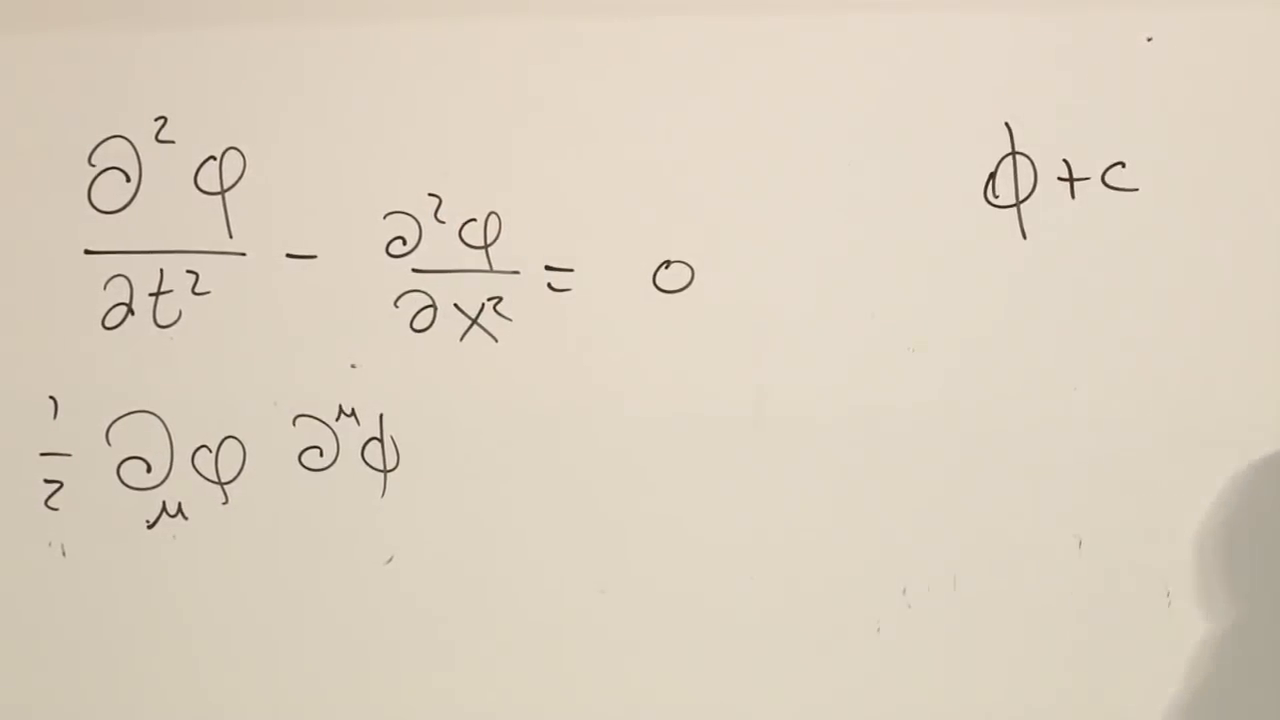
\includegraphics[width=0.90\textwidth]{lecture_07_figure_17.png}
\caption{質量のない波動方程式、その導関数ラグランジアン、および定数シフト\(\phi\mapsto\phi+c\)。}
\lectureframe{01:17:10}
\end{figure}

次に質量項を加える。
\begin{equation}
\frac{\partial^2\phi}{\partial t^2}
-\frac{\partial^2\phi}{\partial x^2}
+\mu^2\phi
=0,
\end{equation}
\begin{equation}
\mathcal L_\mu
=
-\frac12\partial_\mu\phi\,\partial^\mu\phi
-\frac{\mu^2}{2}\phi^2.
\label{eq:sr7-massive-L}
\end{equation}
導関数の部分は
\(\phi\mapsto\phi+c\)の下で変わらないが、\(\phi^2\)は変わらない。どちらの理論も正当であり、一方はシフト不変性を持ち、他方は持たない。

\begin{figure}[htbp]
\centering
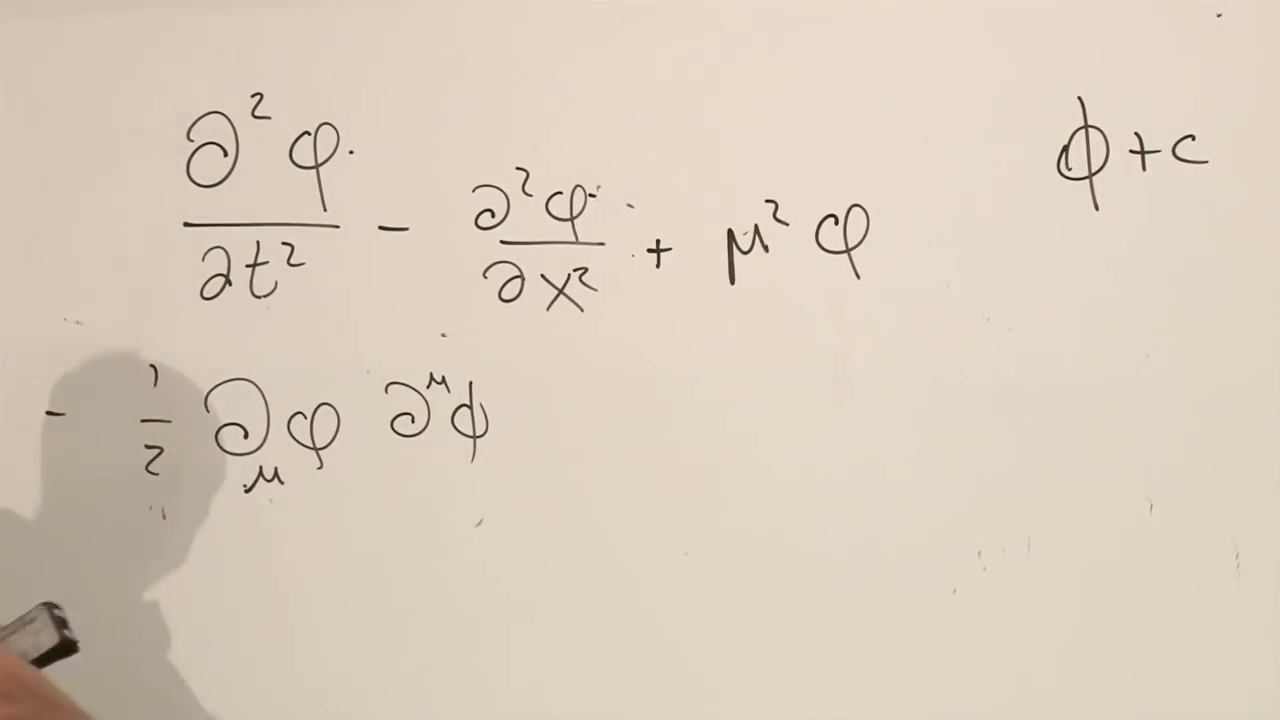
\includegraphics[width=0.90\textwidth]{lecture_07_figure_18.png}
\caption{定数シフト不変性を破る質量項。}
\lectureframe{01:18:50}
\end{figure}

\subsection{学生が境界項を予想する}

聴衆の一人がより鋭いテストを提案する。
\begin{equation}
\phi(x,t)\longrightarrow\phi(x,t)+x.
\label{eq:sr7-linear-shift}
\end{equation}
\(x\)の二階導関数は消えるので、質量のない波動方程式は依然として満たされる。作用はより注意深く見る必要がある。\(x\)と\(t\)は独立変数であるから、
\begin{equation}
\frac{\partial x}{\partial t}=0,
\qquad
\frac{\partial x}{\partial x}=1.
\end{equation}
空間部分は次に従って変化する。
\begin{align}
-\frac12
\left[
\partial_x(\phi+x)
\right]^2
&=
-\frac12
\left(
\partial_x\phi+1
\right)^2
\notag\\
&=
-\frac12(\partial_x\phi)^2
-\partial_x\phi
-\frac12.
\label{eq:sr7-linear-shift-L}
\end{align}
新しい部分は定数と全導関数である。定数はオイラー--ラグランジュ方程式を変えない。\(\partial_x\phi\)を積分すると空間的な境界値のみが生じるので、通常の固定境界条件の下では運動方程式も変わらない。

\begin{figure}[htbp]
\centering
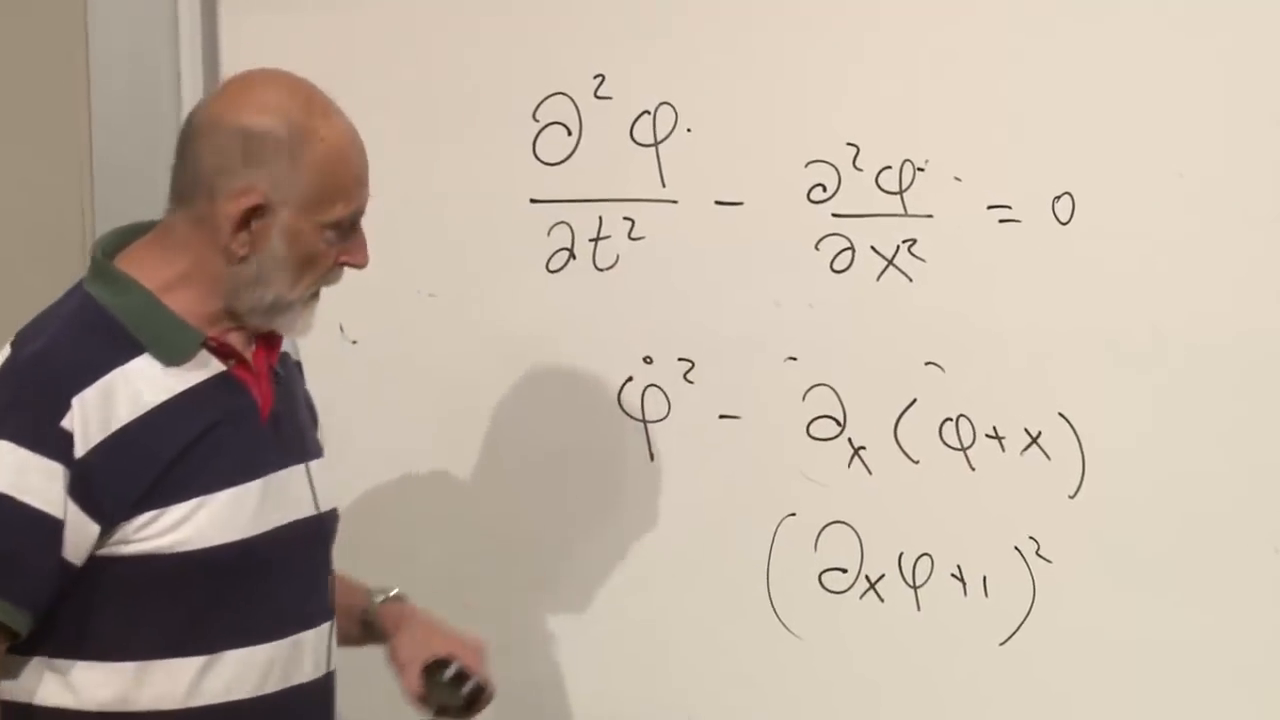
\includegraphics[width=0.90\textwidth]{lecture_07_figure_19.png}
\caption{提案されたシフト\(\phi\mapsto\phi+x\)と、定数と全導関数を明らかにする導関数の二乗。}
\lectureframe{01:22:40}
\end{figure}

\begin{classroomqa}
\audiencequestion{\(\phi\mapsto\phi+x\)はラグランジアン密度を変えるにもかかわらず、質量のない場の方程式を保つか。}
\lecturerresponse{はい。\(x\)の二階導関数は消えるので、方程式は変わらない。ラグランジアンは定数と空間的全導関数だけ変化する。これらは数値的な作用を固定されたバルク定数と境界値だけ変えるが、固定境界条件の下ではオイラー--ラグランジュ方程式は変えない。\lecturetimestamp{01:20:00}}
\end{classroomqa}

\begin{classroomqa}
\audiencequestion{なぜ\(\partial x/\partial t\)はゼロなのか。}
\lecturerresponse{\(x\)と\(t\)は場の記述の独立な座標であるから。\(t\)に関する偏導関数は\(x\)を固定する。\lecturetimestamp{01:22:22}}
\end{classroomqa}

学生は電磁気学に必要な仕掛けに到達した。すなわち、全導関数は書かれた作用を変えても、その停留経路を変えないのである。

\section{荷電粒子のゲージ不変性}

\subsection{四元勾配を加える}

相互作用に戻る
\begin{equation}
I_{\mathrm{int}}
=
-e\int A_\mu\,dx^\mu.
\end{equation}
\(\Lambda(x)\) を任意の十分滑らかなスカラーとし、ポテンシャルを次で変化させる。
\begin{equation}
A_\mu
\longrightarrow
A'_\mu
=
A_\mu+\partial_\mu\Lambda.
\label{eq:sr7-gauge-transformation}
\end{equation}
勾配 \(\partial_\mu\Lambda\) は \(A_\mu\) と同じ共変添字構造をもつので、和は well-defined である。

\begin{figure}[htbp]
\centering
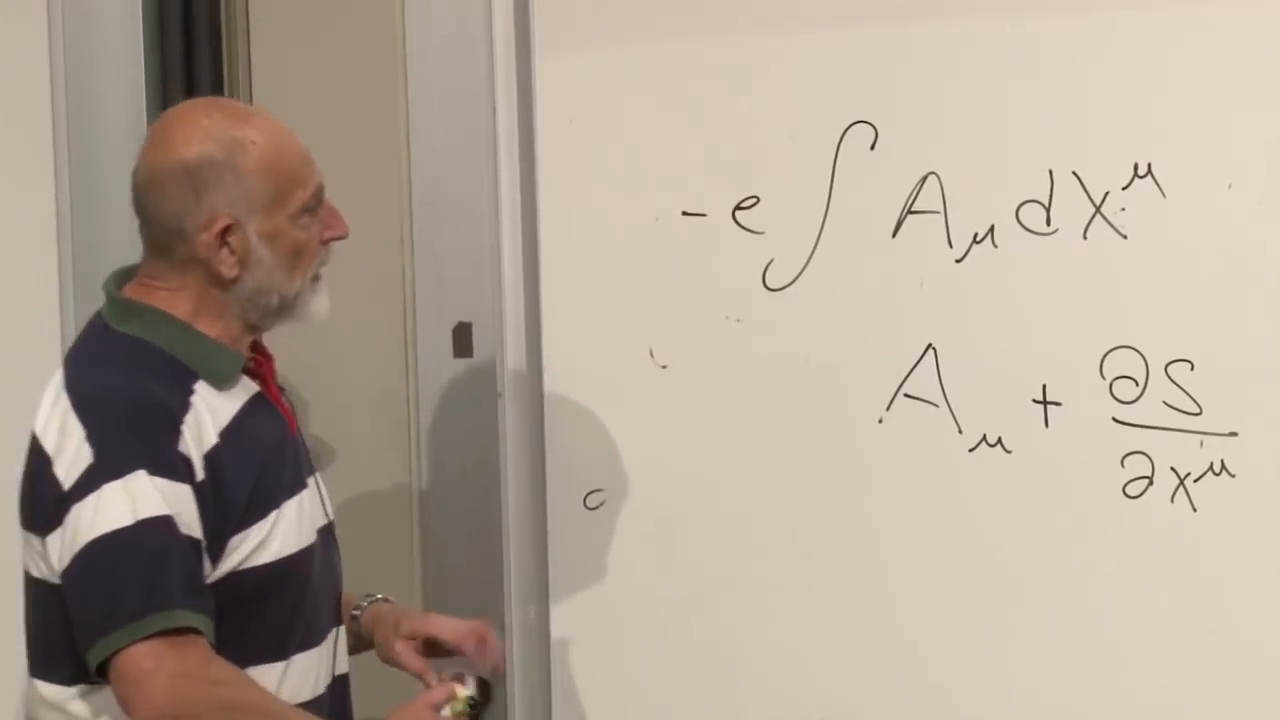
\includegraphics[width=0.90\textwidth]{lecture_07_figure_20.png}
\caption{世界線結合と変換 \(A_\mu\mapsto A_\mu+\partial_\mu\Lambda\)。}
\lectureframe{01:24:50}
\end{figure}

作用の変化は
\begin{align}
\Delta I_{\mathrm{int}}
&=
-e\int \partial_\mu\Lambda\,dx^\mu
\notag\\
&=
-e\int d\Lambda
\notag\\
&=
-e\left[
\Lambda(x_2)-\Lambda(x_1)
\right].
\label{eq:sr7-gauge-boundary}
\end{align}
各無限小世界線区間に沿って、\(\partial_\mu\Lambda\,dx^\mu\) はまさに増分
\(d\Lambda\) である。増分を加え合わせると、終点と始点の値の差に telescoping する。

\begin{figure}[htbp]
\centering
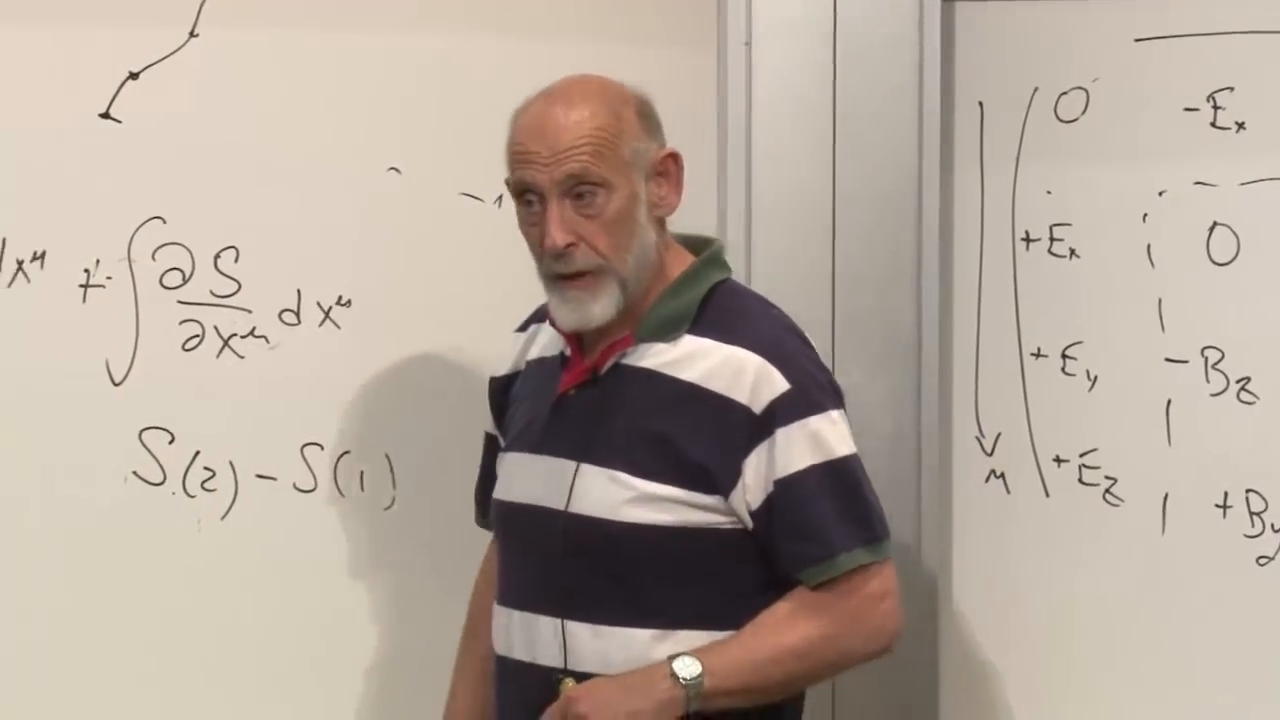
\includegraphics[width=0.90\textwidth]{lecture_07_figure_21.png}
\caption{勾配の寄与は経路に沿って積分され、端点の差 \(\Lambda(x_2)-\Lambda(x_1)\) になる。}
\lectureframe{01:28:10}
\end{figure}

変分原理は、\(x_1\) と
\(x_2\) を固定した近傍の軌道を比較する。したがって \eqref{eq:sr7-gauge-boundary} の余分な項は
許されるどの変分に対しても同じである：
\begin{equation}
\delta\Delta I_{\mathrm{int}}=0.
\end{equation}
停留軌道は変わらない。これが端点の言明としてのゲージ不変性である。

\begin{classroomqa}
\audiencequestion{\(\Lambda\) は任意のスカラー関数でよいか。}
\lecturerresponse{はい。ただし、導関数と作用に必要な滑らかさと境界の仮定を満たす限りにおいてである。この変換が局所的であるのは、パラメータが単なる一つの大域定数ではなく、時空の任意関数だからである。\lecturetimestamp{01:28:40}}
\end{classroomqa}

\(A_\mu\) に勾配を加えることをゲージ変換と呼ぶ。ゲージという語は歴史的な継承物である。講義は、ユーモラスではあるが断固として、フランス語であるかのように発音しないよう警告する。名称は操作よりも重要ではない。

\subsection{場のテンソルによる直接証明}

運動方程式は \(F_{\mu\nu}\) に依存し、ポテンシャルそれ自体には依存しない。\eqref{eq:sr7-gauge-transformation} の下で、
\begin{align}
F'_{\mu\nu}
&=
\partial_\mu
\left(
A_\nu+\partial_\nu\Lambda
\right)
-
\partial_\nu
\left(
A_\mu+\partial_\mu\Lambda
\right)
\notag\\
&=
F_{\mu\nu}
+
\partial_\mu\partial_\nu\Lambda
-
\partial_\nu\partial_\mu\Lambda
\notag\\
&=
F_{\mu\nu}.
\label{eq:sr7-F-gauge-invariant}
\end{align}
通常の平坦な時空における滑らかなスカラーに対しては、偏導関数は可換である。二つの追加項は相殺する。したがって、場のテンソル、それが含む電場と磁場、および力の法則はすべてゲージ不変である。

\begin{figure}[htbp]
\centering
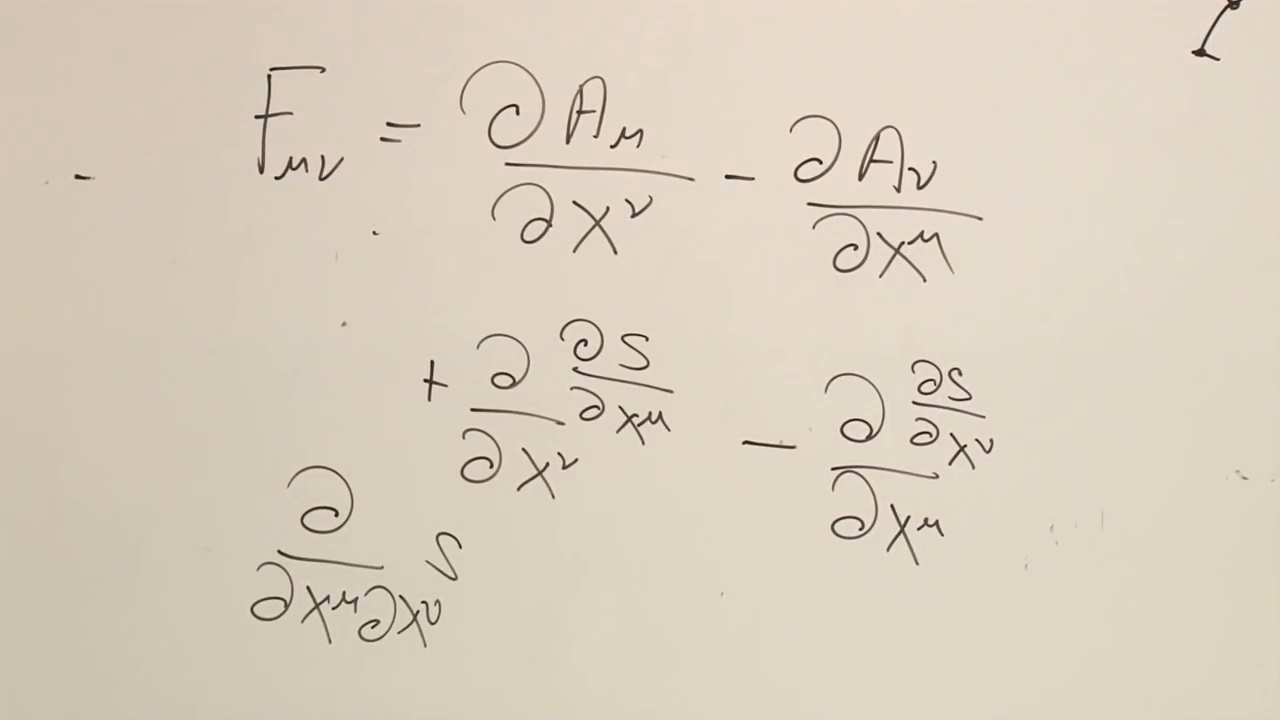
\includegraphics[width=0.90\textwidth]{lecture_07_figure_22.png}
\caption{ゲージ変換から生じる二つの二階導関数は、偏導関数が可換であるために相殺する。}
\lectureframe{01:33:50}
\end{figure}

二つの証明は、反対の方向から同じ円を閉じる。作用は固定された端点でのみ変化し、一方、方程式は変わらない場のテンソルにのみ依存する。

\section{冗長性が意味するもの}

\subsection{なぜ一意でない対象を保持するのか。}

自然な反論はすぐに浮かぶ。\(A_\mu\) が一意でないなら、なぜそれを導入したのか。それは、その成分値が冗長な情報を含んでいても、局所ローレンツ不変な作用に不可欠だからである。多くのポテンシャルが同じ電磁場を表す：
\begin{equation}
A_\mu
\sim
A_\mu+\partial_\mu\Lambda.
\end{equation}
同値類が物理的であり、特定の代表元は記述の選択である。

\begin{classroomqa}
\audiencequestion{ゲージを変えることに実用的な価値はあるか。}
\lecturerresponse{はい。適切な \(\Lambda\) は、ポテンシャルのある成分を簡単にしたり、問題のある特徴を透明にしたりできる。局所的には、そして適切な境界条件の下では、しばしば、\(A_0\) を含む一つの選ばれた成分が消えるようなゲージを選べる。別のゲージは別の特徴をより明瞭に示すかもしれない。\lecturetimestamp{01:35:43}}
\end{classroomqa}

\begin{classroomqa}
\audiencequestion{ゲージ不変性は、同じ実験を二つのローレンツ系から記述することに類似しているか。}
\lecturerresponse{いいえ。ローレンツ変換は、異なる観測者が担う物理的に意味のある基準系を比較する。ゲージ変換は一つの記述内の冗長性である：異なるポテンシャルが同じ場を符号化する。数学的にはどちらも不変性であるが、その解釈は異なる。\lecturetimestamp{01:37:07}}
\end{classroomqa}

構造上の違いもある。回転は固定された大域的な角を用いる；通常、各点で無関係な角だけ軸を回転させることはない。ゲージ変換は関数全体
\(\Lambda(x)\) によってパラメータ化される。この位置依存の自由度が、それを局所ゲージ不変性にしている。

\begin{classroomqa}
\audiencequestion{勾配を加えることがゲージ不変性の一般的定義か。}
\lecturerresponse{アーベル電磁気理論では、それが変換である。Yang--Mills 理論には、ポテンシャルが追加の内部構造を担う、より精巧な非アーベル版があるが、同じ考えは生き残る：異なる局所記述が同じ物理を表す。\lecturetimestamp{01:39:27}}
\end{classroomqa}

\begin{classroomqa}
\audiencequestion{ゲージ変換は、問題の異なる部分を際立たせるための単なる数学的な道具にすぎないのでしょうか。}
\lecturerresponse{それは有用な計算上および解釈上の道具であるが、その役割は制約されている。すなわち、方程式を簡単にしたり、ある性質を明らかにしたりすることはできるが、最終的なゲージ不変な予測を変えることはできない。
\lecturetimestamp{01:40:22}}
\end{classroomqa}

\subsection{他の場と他のポテンシャル}

他の理論におけるゲージポテンシャルも一般に\(A\)で表記され、時空指数\(\mu\)を伴う。それらを区別するのは、他の対称性に付随する追加の内部構造である。講義では、早計な公式を与えるのではなく、その構造を後回しにしている。

\begin{classroomqa}
\audiencequestion{他の場の理論のベクトルポテンシャルはどのようなものですか。}
\lecturerresponse{それらは依然として時空ベクトルとして振る舞い、一般に\(A_\mu\)と書かれるが、内部対称性に付随する追加のラベルと代数的構造を伴う。それがYang--Mills理論への入口であり、意図的に先送りされている。\lecturetimestamp{01:41:02}}
\end{classroomqa}

\begin{classroomqa}
\audiencequestion{局所ローレンツ不変な荷電粒子の作用を、\(\mathbf E\)と\(\mathbf B\)で直接書くことは本当に不可能なのでしょうか。}
\lecturerresponse{ここで述べた仮定の下では、そのとおりである。講義ではこれを定理として提示し、証明はしない。作用原理、局所性、ローレンツ不変性を保つと、ポテンシャルの導入が強制され、その後ゲージ冗長性が自動的に現れる。
\lecturetimestamp{01:42:18}}
\end{classroomqa}

\subsection{何が測定できるのか}

\(A_\mu\)の局所的な値それ自体はゲージ不変ではない。もし物理的測定がその値を一意に決定するなら、それを\(\partial_\mu\Lambda\)だけ変えることは物理的結果を変えることになり、先に証明した不変性に反する。測定可能な予測は、現在の古典的議論における\(F_{\mu\nu}\)のようなゲージ不変量から構成されなければならない。

\begin{classroomqa}
\audiencequestion{なぜ自然はこれほど執拗にゲージ理論を選ぶのでしょうか。}
\lecturerresponse{古典的レベルでは、講義は最終的な理由を与えない。量子力学はより深い視点を提供するが、そこでも広い答えは尽くされていない。すでに明らかなのは、ゲージ冗長性によって組織された理論の並外れた美しさ、対称性、経済性である。
\lecturetimestamp{01:43:36}}
\end{classroomqa}

\begin{classroomqa}
\audiencequestion{ベクトルポテンシャル自体は測定できるのでしょうか。}
\lecturerresponse{ゲージに依存する局所的な成分値としては測定できない。測定は物理的過程であり、すべての物理的予測は\(A_\mu\mapsto A_\mu+\partial_\mu\Lambda\)に鈍感でなければならない。測定できるのは、ポテンシャルと場のゲージ不変な特徴である。
\lecturetimestamp{01:44:18}}
\end{classroomqa}

\begin{classroomqa}
\audiencequestion{\(A_\mu\)が勾配でないものによって変えられたらどうなりますか。}
\lecturerresponse{一般には\(F_{\mu\nu}\)が変わるので、その変化は検出可能である。対照的に、純ゲージポテンシャル\(A_\mu=\partial_\mu\Lambda\)は\(F_{\mu\nu}=0\)を持ち、電磁力を及ぼさない。そのとき自由粒子は直線的な世界線を運動する。\lecturetimestamp{01:45:22}}
\end{classroomqa}

したがってゲージ不変性は使い捨ての技巧ではない。電気力学、Yang--Mills理論、標準模型、重力はすべて、何らかの種類のゲージ冗長性を備えている。そのパターンは特異である。理論を定式化するには補助量が必要だが、その量の一部は物理を変えずに変えることができる。この特異性はまた、組織化の力でもある。

\section{ゲージ不変性の論理}

講義は意図的に遠回りな道をたどってきた。まず上付き--下付きの言語を復元した。スカラー縮約がローレンツ不変な作用の文法だからである。次に四つの原理を述べた。作用、局所性、ローレンツ不変性、ゲージ不変性である。第四のものは、荷電粒子の計算を再構築する間、未定義のままにされた。

その計算は局所スカラー作用
\begin{equation}
I
=
-m\int d\tau
-e\int A_\mu dx^\mu,
\end{equation}
から始まり、通常時間のラグランジアンとすべてのEuler--Lagrange微分を経て、電気的および磁気的ローレンツ力を再現した。次に固有時間が結果を
\begin{equation}
m\frac{du^\mu}{d\tau}
=
-eF^\mu{}_\nu u^\nu,
\qquad
F_{\mu\nu}
=
\partial_\mu A_\nu-\partial_\nu A_\mu.
\end{equation}
に組み立てた。

スカラー場の例は最終段階を準備した。全微分は境界を通じてのみ作用を変えうる。したがって、
\begin{equation}
A_\mu\longrightarrow A_\mu+\partial_\mu\Lambda
\end{equation}
は世界線作用を固定された端点の値だけ変え、混合偏微分が可換であるため\(F_{\mu\nu}\)を変えない。よってベクトルポテンシャルは必要だが一意ではない。ゲージ不変性とは、この非一意性が物理ではなく記述に属するという主張である。